% !Mode:: "TeX:UTF-8"
%%%%%%%%%%%%%%%%%%%%%%%%%%%%%%%%%%%%%%%%%%%%%%%%%%%%%%%%%%%%%%%%%%%%%%%%%%%%%%%%
%          ,
%      /\^/`\
%     | \/   |                CONGRATULATIONS!
%     | |    |             SPRING IS IN THE AIR!
%     \ \    /                                                _ _
%      '\\//'                                               _{ ' }_
%        ||                     heuthesis v31                { `.!.` }
%        ||                                                ',_/Y\_,'
%        ||  ,                                               {_,_}
%    |\  ||  |\            Email: lwh@hrbeu.edu.cn             |
%    | | ||  | |          https://www.hrbeu.edu.cn           (\|  /)
%    | | || / /                                               \| //
%    \ \||/ /       https://gitee.com/liwenhui/heuthesis      |//
%      `\\//`   \\   \./    \\ /     //    \\./   \\   //   \\ |/ /
%     ^^^^^^^^^^^^^^^^^^^^^^^^^^^^^^^^^^^^^^^^^^^^^^^^^^^^^^^^^^^^^^
%%%%%%%%%%%%%%%%%%%%%%%%%%%%%%%%%%%%%%%%%%%%%%%%%%%%%%%%%%%%%%%%%%%%%%%%%%%%%%%%
\documentclass[type=postdoc]{heuthesisbook}
% 此处选项中不要有空格
%%%%%%%%%%%%%%%%%%%%%%%%%%%%%%%%%%%%%%%%%%%%%%%%%%%%%%%%%%%%%%%%%%%%%%%%%%%%%%%%
% 必填选项
% type=doctor|master|bachelor|postdoc
%%%%%%%%%%%%%%%%%%%%%%%%%%%%%%%%%%%%%%%%%%%%%%%%%%%%%%%%%%%%%%%%%%%%%%%%%%%%%%%%
% 选填选项(选填选项的缺省值已经尽可能满足了大多数需求,除非明确知道自己有什么
% 需求)
% tocfour=true|false
%   含义:是否添加第四级目录,只对本科文科个别要求四级目录有效,缺省值为
%   false
% subtitle=true|false
%   含义:论文题目是否含有副标题,缺省值为false,如果有要在cover中设置副标
%   题内容,封面中显示。
% openright=true|false
%   含义:博士论文是否要求章节首页必须在奇数页,此选项不在规范要求中,按个
%   人喜好自行决定。 默认否。注意,我校的默认情况是打印版博士论文要求右翻页
%   ,电子版要求非右翻页且无空白页。如果想DIY(或身不由己DIY)在什么地方右
%   翻页,将这个选项设置为false,然后在目标位置添加`\cleardoublepage`命令即
%   可。
% engtoc=true|false
%   含义:是否需要添加英文目录
%%%%%%%%%%%%%%%%%%%%%%%%%%%%%%%%%%%%%%%%%%%%%%%%%%%%%%%%%%%%%%%%%%%%%%%%%%%%%%%%
\usepackage{heuthesis}

\graphicspath{{figures/}}

\begin{document}
\frontmatter
% !Mode:: "TeX:UTF-8"

\heusetup{
  %******************************
  % 注意:
  %   1. 配置里面不要出现空行
  %   2. 不需要的配置信息可以删除
  %******************************
  %
  %=========
  % 秘级编号
  %=========
  statesecrets={公开},          %密级
  cnumber={no9527},             %编号
  natclassifiedindex={TM301.2}, %分类号
  intclassifiedindex={62-5},    %UDC编号
  %
  %=========
  % 中文信息
  %=========
  ctitlecover={基于~\LaTeX~的哈尔滨工程大学本硕博\\论文模板使用说明}, %放在封面中使用,在需要换行的地方插入\\
  ctitle={基于~\LaTeX~的哈尔滨工程大学本硕博论文模板使用说明},        %页眉使用论文标题,不换行
  csubject={动力工程及工程热物理}, %专业
  caffil={动力与能源工程学院},     %所在单位/学院
  cauthor={马冬梅},                %论文作者
  csupervisor={孔夫子},            %指导老师
  cprofessional={教授},            %指导老师职称
  csupervisorcaffil={动力与能源工程学院}, %导师单位
  % 日期自动使用当前时间,若需指定按如下方式修改:
  %cdate={超新星纪元}, %封面日期,不指定使用当前日期
  csubmitdate={20XX年XX月}, %提交日期
  coralexdate={20XX年XX月}, %答辩日期
  cstudentid={202103123},   %学号
  %
  %=========
  % 英文信息
  %=========
  etitle={Manual of~ \LaTeX ~Thesis Template of\\ Harbin Engineering University}, %论文题目(英文),在需要换行的地方插入\\
  %
  % 中英文关键词,用“英文逗号(,)”分割
  ckeywords={\TeX, \LaTeX, 论文, 模板},
  ekeywords={\TeX, \LaTeX, template, thesis},
}

\begin{cabstract}
  摘要的字数(以汉字计),本科、硕士学位论文一般为500 $\sim$ 1000字,博士学位论文为1000 $\sim$ 2000字,
  均以能将规定内容阐述清楚为原则,文字要精练,段落衔接要流畅。摘要页不需写出论文题目。
  英文摘要与中文摘要的内容应一致,在语法、用词上应准确无误,语言简练通顺。

  关键词是为了文献标引工作、用以表示全文主要内容信息的单词或术语。关键词不超过 5
  个,每个关键词中间用分号分隔。(关键词分隔符不用考虑,模板会自动处理。英文关键词同理。)
\end{cabstract}

\begin{eabstract}
  An abstract of a dissertation is a summary and extraction of research work
  and contributions. Included in an abstract should be description of research
  topic and research objective, brief introduction to methodology and research
  process, and summarization of conclusion and contributions of the
  research. An abstract should be characterized by independence and clarity and
  carry identical information with the dissertation. It should be such that the
  general idea and major contributions of the dissertation are conveyed without
  reading the dissertation.

  An abstract should be concise and to the point. It is a misunderstanding to
  make an abstract an outline of the dissertation and words “the first
  chapter”, “the second chapter” and the like should be avoided in the
  abstract.

  Key words are terms used in a dissertation for indexing, reflecting core
  information of the dissertation. An abstract may contain a maximum of 5 key
  words, with semi-colons used in between to separate one another.
\end{eabstract}

 % 封面
\makecover

\tableofcontents %目录

%%----------  插图目录, 如不需要可用 % 注释掉下面两行
\listoffigures
\cleardoublepage

%%----------  表格目录, 如不需要可用 % 注释掉下面两行
\listoftables
\cleardoublepage

\mainmatter
% !Mode:: "TeX:UTF-8"

\chapter[哈尔滨工程大学研究生学位论文规范]{哈尔滨工程大学研究生学
  位论文\protect\\规范}[Harbin Engineering University Postgraduate Dissertation Writing Specifications]

\section{引言}[Introduction]

学位论文是表明作者从事科学研究取得创造性结果或有了新的见解,并以此为内容撰写而成的学术论文。研究生学位论文展示了研究生在科学研究工作中取得的成果并全面反映了研究生对本学科基础理论和专门知识的掌握程度,是申请和授予相应学位的基本依据。学位论文撰写是研究生培养过程的基本训练之一,必须按照确定的规范认真执行。

本论文规范按照《科学技术报告、学位论文和学术论文的编写格式》(GB 7713-87)、《文后参考文献著录规则》(GB 7714-87)以及《标准化工作导则标准编写的基本规定》(GB/T1.1-1993)制定。

本论文规范适用于我校博士、硕士研究生(工商管理硕士学位论文规范已经规定的内容除外)和以研究生毕业同等学力在我校申请博士、硕士学位的在职人员。博士和硕士学位论文除在字数、理论研究的深度及创造性成果等方面的要求不同以及特殊说明外,对其撰写规范的要求基本一致。


\section{基本要求}[Content specification]

\subsection{撰写依据}[Writing Based]

除论文的语言文字须符合汉语语法规范外,论文撰写应符合国家及各专业部门制定的有关标准。在本规范的“附录A 相关标准”中列出了一些常用标准。

\subsection{论文字数}[Words Required]

博士学位论文,理工类学科:6-8万字,管理及人文学科:8-10万字。

硕士学位论文,理工科:3-4万字,管理及人文学科:4-5万字。

\subsection{论文结构及各部分要求}[Struct Required]

请参见“附录F学位论文结构图”

\subsubsection{前置部分}[Front Parts]

前置部分包括封面、扉页、论文原创性声明、摘要、目录、插图和附表清单。

论文题目要恰当、准确地反映本论文的研究内容。摘要应包括本论文的创造性成果及其理论与实际意义。为了便于国际交流,扉页、摘要、关键词应有中英文两种。插图和附表清单不是必选项,只在图表较多时使用。

\subsubsection{论文主体部分}[Paper Body]

论文主体部分一般包括绪论(引言)、正文、结论、参考文献、攻读学位期间发表的论文和取得的科研成果、致谢、个人简历(个人简历仅对在职人员和在职研究生要求)。

主体部分是学位论文的核心,由于研究工作涉及的学科、选题、研究方法、工作进程、结果表达等有很大差异,故不对主体部分中论文正文内容作统一规定。但要求明确指出本论文的创新点或实际应用之处。文中引用的他人研究成果部分单独书写,并注明出处,不得将其与本人提出的理论分析混淆在一起。论文主体部分要求逻辑清晰,层次分明,实事求是,简练可读。

建议包含以下内容:总体研究方案设计与选择论证、实验和观测方案设计的可行性,有效性和数据处理及分析、理论分析。

\subsubsection{附录部分(必要时)}[Appendix]

对需要收录于学位论文中且又不适合书写于正文中的附加数据、资料、详细公式推导等有助于读者理解学位论文的内容,可作为附录。

\subsubsection{结尾部分(可以没有)}[End Part]

结尾部分可以提供有关输入数据和索引。

\section{具体编写格式}[Format Details]

\subsection{封面}[Cover]

封面是学位论文的外表面,提供应有的信息,并起到保护作用。封面包含以下内容:

a.分类号 \quad 在左上角注明《中国图书资料分类法》的类号和《国际十进分类法UDC》的类号。

b.密级和编号 \quad 若论文内容属保密范围,按国家规定的保密条例,在右上角注明密级,并注明为正本或副本。如系公开发行,不注密级。

c.论文题目 \quad 论文题目名称应恰当、准确地反映本论文的研究内容。学位论文的中文题名不宜超过20字,并尽量不设副标题。题名应标注于封面偏上正中位置,并在其正上方注明“\uline{\qquad}”士学位论文字样(“\uline{\qquad}”指所获硕士或博士学科门类,如管理学硕或管理学博)。若作者为在职人员以同等学力申请学位还应在上述文字和论文题目之间注明“(在职人员)”字样。

d.作者姓名。“

e.导师姓名、专业技术职务 \quad 专业技术职务不可简写。

f.学科、专业名称 \quad 按二级学科填写,若为一级学科博士学位授权专业或该一级学科不设二级学科则按一级学科填写。

g.学位授予单位 \quad 在封面下部居中写明学位授予单位“哈尔滨工程大学”。

\subsection{扉页}[Second Page]

扉页提供整个学位论文有关信息的详细说明,扉页包含封面中的各项内容,并且还包括以下内容:

a.申请学位级别 \quad 应写明学科门类、学位级别

b.论文提交日期

c.论文答辩日期

d.作者所在单位 \quad 本校学生填所在院(系),同等学力申请学位人员
或在职研究生填写本人所在单位。

英文扉页不注密级和编号,其他内容与相应中文内容一致。

\subsection{摘要}[Abstraction]

摘要是学位论文内容的简短陈述,应具有独立性和自含性,即不阅读全文就能获得必要信息。摘要内容要说明研究工作目的、实验方法、结果和最终结论,重点是结果和结论。除实在无变通办法可用以外,摘要中不使用图、表、化学结构式、特殊符号和术语,不标注引用文献号。要求中、英文摘要内容要一致。

\subsection{关键词}[Keywords]

关键词是供检索用的主题词条,应采用能覆盖论文主要内容的通用技术词条(参照相应的技术术语标准)。关键词一般列3-5个,按词条外延层次排列(外延大的排在前面)。英文关键词与中文关键词要求相同。

\subsection{目录}[Content]

目录应包括论文中全部章节的标题及页码,含:
章节题目(要求编到第3级标题,即X.X.X)
参考文献
攻读X士学位期间发表的论文和取得的科研成果
致谢
个人简历(仅对在职人员和在职研究生要求有此要求)
附录(可选项)
索引(可选项)

\subsection{插图和附表清单(可选择)}[Graphics Index]

如果论文中图表较多,可以分别列出清单置于目录之后。图的清单应有序号、图题和页码。表的清单应有序号、表题和页码。

\subsection{章节编排}[Section Arrange]

论文主体部分分章节撰写,每章另起一页。除绪论(引言)外正文每一章后应有一节“本章小结”。绪论(引言)一般作为第一章,结论、参考文献、攻读学位期间发表的论文和取得的科研成果、致谢、个人简历、附录、索引不编排章号。

各章标题要突出重点、简明扼要。字数一般在15字以内,不得使用标点符号。标题中尽量不采用英文缩写词,对必须采用者,应用使用本行业通用缩写词。

章、条的编号参照国家标准GB1.1《标准化工作导则标准编写的基本规定》第8章“标准条文的编排”的有关规定,采用阿拉伯数字分级编号,
即1、1.1、1.1.1……的形式。层次一般不大于四级。

\subsection{绪论(引言)}[Introduce]

绪论(引言)简要说明研究工作的目的、范围、相关领域的前人工作和知识空白、理论基础和分析、研究设想、研究方法和实验设计、预期结果和意义等。

\subsection{正文}[Main Body]


\subsubsection{编码}[Index No]

正文中的图、表、附注、参考文献、公式、算式等一律用阿拉伯数字分章依序连续编排序号或就全文统一依序编排。其标注形式为:图2.1、表3.2;附注1);文献[4];式(3-5)等。

\subsubsection{数字}[Number]

按国家语言学工作委员会等七单位1987年发布的《关于出版物上数字用法的试行规定》,一般采用阿拉伯数字。

\subsubsection{公式}[Fomular]

正文中的公式应居中书写。若公式前有文字,空两格写文字,公式居中写。公式末尾不加标点。

公式序号按章编排,用阿拉伯数字,序号写在右边,并加圆括号,如第一章第一个公式号为“(1-1)”,附录A中的第一个公式为(A1)等。

文中引用公式时,一般用“见式(1-1)”或“由公式(1-1)”。

较长公式必须转行时,只能在等号(=)或加(+)、减(-)、乘()、除(÷)等运算符号后断开转行,上下行尽可能在等号处对齐。

公式中符号的含义和计量单位应注释在公式的下面。每条注释应另行书写,移行时,与其开始写文字的位置对齐。

例:第一章第一个公式:

\begin{equation}\label{form2x1}
  f=\frac{1}{2\pi\sqrt{LC}}
\end{equation}

\begin{tabularx}{\textwidth}{@{}l@{\quad}r@{——}X@{}}
式中 & $\boldsymbol{f}$    & 频率,MHz; \\
	 & $\boldsymbol{L}$    & 电感量,H;  \\
 	 & $\mathbf{C}$        & 电容量,pF。                       
\end{tabularx}\vspace{3.15bp}

\subsubsection{插图}[Pictures]

插图包括曲线图、构造图、示意图、图解、框图、流程图、记录图、布置图、地图、照片等。

第一图应有简短确切的题名,连同图序置于图下,图名中不允许使用标点符号,图名后不加标点符号。图序与图名之间空一格。博士学位论文还应在中文图名下注明相应的英文图名。

插图应与正文的内容紧密配合,插图和有关图形符号符合制图、图形符等有关标准规定。插图应具有“自明性”,即只看图、图题和图例,不阅读正文就可理解图意。必要时,应将图上的符号、标记、代码以及实验条件等,用最简练的文字,横排于图题下方,作为图例说明。

插图的纵横坐标必须标注“量、标准规定符号、单位”。此三者只有在不必要标明(如无量纲等)的情况下方可省略。坐标上标注的量的符号和缩略词必须与正文中的一致。

表示函数关系的曲线图,如有确定曲线的函数式,则应在有关条文中,或在图的下方,或在图中适当位置写出。曲线图内,不应有过多的空白,如果曲线不占其整个面积,应当将图截短,只保留有曲线的坐标部分。

若条件允许,插图要用相应的计算机绘图软件绘制。

每一图应有简短确切的题名,连同图号置于图下。

\subsubsection{插表}[Table]

表序与表名书写于表的正上方,表序与表名之间空一格,表名不允许使用标点符号,表名后不加标点。博士学位论文还应在表名下注明相应的英文表名。

表格的上部和下部用粗实线闭合,左、右两侧不加竖线闭合。在表格横向狭而长,排版时幅面宽度不够时,可将表格分为两段,用细双线接排在一页内。(见\ref{tab:tbl-1-1} - \ref{tab:tbl-1-3})。

表格中各栏参数的计量单位相同时,应将单位写在表的右上角(见表3.1);如计量单位不同时,应将单位分别写在各栏参数名称的下方。若相邻参数采用相同的单位时,可合并写在它们共同的单位栏内(见表3.2);如表格中大多数的计量单位相同,可将该单位写在右上角,将其余的少数单位写在有关栏内(见表3.3)。

当插表太宽,无法在该页横排时,可以逆时针方向旋转90度放置。

% Table generated by Excel2LaTeX from sheet 'Sheet1'
\begin{table}[htbp]
  \centering\wuhao
  \caption{横向长标示例}\hspace{100mm}mm\\
  \begin{tabular}{p{4.0em}cccccc}
    \toprule
    \multicolumn{1}{c}{} & \multicolumn{1}{p{4.0em}}{a}  & \multicolumn{1}{p{4.0em}}{b} & \multicolumn{1}{p{4.0em}}{c} & \multicolumn{1}{p{4.0em}}{d} & \multicolumn{1}{p{4.0em}}{e} & \multicolumn{1}{p{4.0em}}{f} \\
    \midrule
    A                    &                               &                              &                              &                              &                              &                              \\
    B                    &                               &                              &                              &                              &                              &                              \\
    \midrule
    \midrule
    \multicolumn{1}{c}{} & \multicolumn{1}{p{4.0em}}{g } & \multicolumn{1}{p{4.0em}}{h} & \multicolumn{1}{p{4.0em}}{i} & \multicolumn{1}{p{4.0em}}{j} & \multicolumn{1}{p{4.0em}}{k} & \multicolumn{1}{p{4.0em}}{l} \\
    \midrule
    A                    &                               &                              &                              &                              &                              &                              \\
    B                    &                               &                              &                              &                              &                              &                              \\
    \bottomrule
  \end{tabular}%
  \label{tab:tbl-1-1}%
\end{table}%

% Table generated by Excel2LaTeX from sheet 'Sheet2'
\begin{table}[htbp]
  \centering\wuhao
  \caption{表格示例1}
  \vspace{0.5em}
  \begin{tabular}{cccccccc}
    \toprule
    \multicolumn{1}{c}{\multirow{2}[4]{*}{m/t}} & \multicolumn{1}{c}{\multirow{2}[4]{*}{H/m}} & \multicolumn{1}{p{4.0em}}{B}    & \multicolumn{1}{p{4.0em}}{K}  & \multicolumn{1}{p{4.0em}}{L} & \multicolumn{1}{p{4.0em}}{H1} & \multicolumn{1}{p{4.0em}}{H} & \multicolumn{1}{p{4.0em}}{轮压} \\
    \cmidrule{3-8}                              &                                             & \multicolumn{5}{p{20.95em}}{Mm} & \multicolumn{1}{p{4.0em}}{Pa}                                                                                                                                 \\
    \midrule
                                                &                                             & \multicolumn{5}{c}{}            &                                                                                                                                                               \\
    \bottomrule
  \end{tabular}%
  \label{tab:tbl-1-2}%
\end{table}%

% Table generated by Excel2LaTeX from sheet 'Sheet3'
\begin{table}[htbp]
  \centering\wuhao
  \caption{表格示例2}
  \vspace{0.5em}
  \begin{tabular}{p{2.6em}p{2.6em}p{2.6em}ccccp{3.2em}}
    \toprule
    \multirow{2}[4]{*}{规格} & \multirow{2}[4]{*}{A} & \multirow{2}[4]{*}{B} & \multicolumn{2}{c}{H} & \multicolumn{2}{c}{L} & \multirow{2}[4]{*}{m/Kg}                    \\
    \cmidrule{4-7}           &                       &                       & 基本尺寸              & 极限偏差              & 基本尺寸                 & 极限偏差 &       \\
    \midrule
    100                      & 100                   & -                     & 4                     &                       & 10                       & ±0.3     & 8.5   \\
    200                      & 150                   & 20                    & 6                     & ±0.1                  & 50                       & ±0.4     & 23.5  \\
    300                      & 200                   & 30                    & 10                    &                       & 70                       & ±0.5     & 75.6  \\
    400                      & -                     & 40                    & 15                    &                       & 100                      & ±.06     & 120.7 \\
    \bottomrule
  \end{tabular}%
  \label{tab:tbl-1-3}%
\end{table}%

表格中各栏参数的计量单位相同时,应将单位写在表的右上角(见表\ref{tab:tbl-1-1});如计量单位不同时,应将单位分别写在各栏参数名称的下方。若相邻参数采用相同的单位时,可合并写在它们共同的单位栏内(见表3.2);如表格中大多数的计量单位相同,可将该单位写在右上角,将其余的少数单位写在有关栏内(见表3.3)。

当插表太宽,无法在该页横排时,可以逆时针方向旋转90度放置。

\subsubsection{文献引用形式}[Reference Style]

引用文献标示应置于所引内容最末句的右上角,用小五号字体。所引文献编号用阿拉伯数字置于方括号“[]”中。当提及的参考文献为文中直接说明时,文献编号置于方括号中与正文排齐,字号大小与正文相同。

\subsubsection{科技术语和缩略词}[Terms and abbreviations]

科技术语和缩略词应采用国家标准。标准中未规定的要按本学科或本专业的权威性机构或学术团体公布的规定执行。全文名词术语必须统一。首次出现的特殊科技术语和缩略词应在适当位置加以说明或注解。

\subsubsection{物理量名称和符号}[Physical quantity name and symbol]

物理量名称和符号应符合国标GB1434-78《物理量符号》、GB3100-82《国际单位制及其应用》、GB3101-82《有关量、单位和符号的一般原则》、GB3102.1-1993到GB3102.13-1993(名称请见附录A)的规定,论文中某一物理量的名称符号应统一。

\subsubsection{物理量计量单位(打印)}[Physical quantity UOM]

计量单位及符号必须采用1984年2月27日国务院发布的《中华人民共和国法定计量单位》并遵照《中华人民共和国法定计量单位使用方法》执行。

\subsubsection{外文字母的正、斜体用法}[外文字母的正、斜体用法]

按照GB3100~3102-1993(名称请见附录A)及GB7159-87 电气技术中的文字符号设计通则的规定使用,即物理量符号、物理常量、变量符号用斜体,计量单位等符号均用正体。$sin{x}$、$cos{x}$等三角函数应用正体。

\subsection{结论}[conclusion]

结论是论文最终的、总体的结论,不是正文中各段的小结的简单重复。
在结论中应明确指出本研究内容的创造性成果或创新点理论(含新见解、新观点),对其应用前景和社会、经济价值等加以预测和评价,及其今后进一步进行研究工作的展望与设想。结论应该准确、完整、明确、精练。

\subsection{致谢}[thanks]

致谢内容应该简洁明了、实事求是。

\subsection{参考文献}[reference]

参考文献书写格式应符合GB7714-87《文后参考文献著录规则》。若同一文献中有多处被引用,则要写出相应引用页码,各起止页码间空一格,排列按引用顺序,不按页码顺序。常用参考文献编写项目和顺序规定如下,(其中版次为第一版的要省略版次):

著作图书文献

序号 \quad 作者.书名.版次.出版者,出版年:引用部分起止页

翻译图书文献

序号 \quad 作者.书名.译者.版次.出版者,出版年:引用部分起止页

学术刊物文献

序号 \quad 作者.文章名.学术刊物名.年,卷(期):引用部分起止页

学术会议文献

序号 \quad 作者.文章名.编者名.会议名称,会议地址,年份.出版地:出版者,出版年:引用部分起止页

学位论文类参考文献

序号 \quad 研究生名.学位论文题目.学校及学位论文级别.答辩年份:引用部分起止页

学术会议若出版论文集者,可在会议名称后加上“论文集”字样。未出版论文集者省去“出版者”、“出版地”、“出版年”三项。会议地址与出版地相同者省略“出版地”。会议年份与出版年相同者省略“出版年”。

产品说明书、各类标准、各种报纸上刊登的文章及未公开发表的研究报告不宜作为参考文献。

\subsection{攻读XX学位期间发表的论文和取得的科研成果}[Publications]

攻读学位期间发表的论文格式与参考文献相同。取得的科研成果格式为:

a.获奖项目名称 \quad 奖励名称 \quad 级别 \quad 日期 \quad 排名

b.获专利名称 \quad 专利号 \quad 专利所在国家和专利类别 \quad 日期 \quad 排名

\textbf{注意:不论有无发表的论文和取得的科研成果,本章不能省略。}

\subsection{个人简历}[Resume]

仅对同等学力申请学位人员和在职研究生要求。

个人简历应包含取得各级学位的时间和地点、担任各种职务的时间和任职单位、参加过的科研工作和取得的成果。

\subsection{附录}[Appendix]

附录是论文主体部分的补充项目,视论文需要决定是否使用。

对需要收录于学位论文中,但又不便书写于正文中的附加数据、资料、详细公式推导等有特色的内容,可做为附录。每一附录均另页起,论文的附录依序用大写正体A,B,C,……编序号,如:附录A。附录中的图、表、式、参考文献等另行编序号,与正文分开,也一律用阿拉伯数字编码,但在数码前冠以附录序码,如:图A1;表B2;式(B3);文献[A5]等。

\subsection{索引}[Index]

为便于检索文中内容,可编制索引置于论文之后,索引不是必需的项目。索引以论文中的专业词语为检索线索,指出其相关内容的所在页码。索引用中、英两种文字分别书写,中文在前。中文按各词汉语拼音第一个字母排序,英文按该词第一个英文字母排序。

\section{打印要求}[Print Requirement]

研究生学位论文一律要求用计算机打印,并尽量用流行的排版软件。

我校各级研究生学位论文(含专业学位论文以及涉密学位论文)的版面一律改成A4纸,页边距上、下设置为28mm,左、右设置为25mm,页眉、页脚设置为20mm。装订时上、下、右各切除3mm,学位论文成品版面大小为207mm*291mm。

\subsection{字体与字号}[Font and Size]

各章题序及标题:小2号黑体;

各节的一级题序及标题:小3号黑体;

各节的二级题序及标题:4号黑体;

各节的三级题序及标题:小4号黑体;

款、项:均采用小4号黑体;

正文用小4号宋体。

摘要、结论、参考文献、致谢、攻读学位期间发表的论文和取得的科研成果、个人简历等部分按章处理,即标题小2号黑体,内容小4号宋体。目录的标题采用小2号黑体,内容中章的标题用小4号黑体,其它为小4号宋体。

\subsection{页码}[Page Number]

论文页码一律用阿拉伯数字连续编码。页码由第1章的首页开始,作为第1页。论文前置部分(封面、扉页、摘要、目录、插图和附表清单)不编排页码。页码位于整页下部居中。封面、扉页为右页且为单面页。摘要、目录、插图和附表表单、各章、结论、参考文献、攻读xx学位期间发表的论文和取得的科研成果、致谢、个人简历另起一页。

\subsection{页眉与页脚}[Page Head and Foot]

论文不加页脚。论文的封面、扉页、不加页眉,其它部分均加页眉。页眉采用宋体5号字居中放置,若论文为双面印刷,则奇、偶页页眉内容不同。奇数页为本页内容所属的章的题目,即“第n章 ”的形式,若本页含的内容不编章号,则页眉为本学位论文的题目;偶数页为“哈尔滨工程大学 \underline{\hspace{1em}} 士学位论文”( \underline{\hspace{1em}} 为“硕”或“博”)。若论文为单面印刷,则奇、偶页内容相同一律为“哈尔滨工程大学 \underline{\hspace{1em}} 士学位论文”。页眉下划线要求为双线,上细下粗。细线粗约0.5mm,粗线约0.8mm,粗线与细线间距约为0.3mm。

\subsection{封面}[Cover]


\subsection{扉页(内封)}[Second Page]


\subsection{摘要及关键词}[Abstract and Key Words]

摘要题头应居中,然后隔行书写摘要的文字部分。摘要文字之后隔一行写关键词,格式见样例。

\subsection{印刷和装订}[Print and Binging]

硕士、博士学位论文原件要求与计算机程序清单、实验原始记录等与论文有关的材料装订在一起。

硕士学位论文的封面采用“绿丝棉”纸,博士学位论文封面均采用“莱妮纹”纸(克重:200gsm,颜色:银灰色)。

书脊处应印刷论文题目及“哈尔滨工程大学 \underline{\hspace{1em}} 士学位论文”(\underline{\hspace{1em}} 为“博”或“硕”)字样,字体用适当字号的宋体字。



% Local Variables:
% TeX-master: "../thesis"
% TeX-engine: xetex
% End:
% !Mode:: "TeX:UTF-8"

\chapter{示例文档}[Example]

这是 \heuthesis\ 的示例文档,基本上覆盖了模板中所有格式的设置。建议大家在使用模
板之前,除了阅读《\heuthesis\:哈尔滨工程大学学位论文模板》\footnote{即
  heuthesis.pdf文件},本示例文档也最好能看一看。此示例文档尽量使用到所有的排版格式
,然而对于一些不在我校规范中规定的文档,理论上是由用户自由发挥,这里不给出样例
。需要另行载入的宏包和自定义命令在文件`heuthesis.sty'中有示例,这里不列举。

\section{关于数字}[Number]

按《关于出版物上数字用法的试行规定》(1987年1月1日国家语言文字工作委员会等7个单位公布),除习惯用中文数字表示的以外,一般数字均用阿拉伯数字。\par
(1)公历的世纪、年代、年、月、日和时刻一律用阿拉伯数字,如20世纪,80年代,4时3刻等。年号要用四位数,如1989年,不能用89年。\par
(2)记数与计算(含正负整数、分数、小数、百分比、约数等)一律用阿拉伯数字,如3/4,4.5\%,10个月,500多种等。\par
(3)一个数值的书写形式要照顾到上下文。不是出现在一组表示科学计量和具有统计意义数字中的一位数可以用汉字,如一个人,六条意见。星期几一律用汉字,如星期六。邻近两个数字并列连用,表示概数,应该用汉字数字,数字间不用顿号隔开,如三五天,七八十种,四十五六岁,一千七八百元等。\par
(4)数字作为词素构成定型的词、词组、惯用语、缩略语等应当使用汉字。如二倍体,三叶虫,第三世界,“七五”规划,相差十万八千里等。\par
(5)5位以上的数字,尾数零多的,可改写为以万、亿为单位的数。一般情况下不得以十、百、千、十万、百万、千万、十亿、百亿、千亿作为单位。如~\num{345000000}~公里可改写为3.45亿公里或~\num{34500}~万公里,但不能写为3亿~\num{4500}~万公里或3亿4千5百万公里。\par
(6)数字的书写不必每格一个数码,一般每两数码占一格,数字间分节不用分位号“,”,凡4位或4位以上的数都从个位起每3位数空半个数码(1/4汉字)。“\num{3000000}”,不要写成“3,000,000”,小数点后的数从小数点起向右按每三位一组分节。一个用阿拉伯数字书写的多位数不能从数字中间转行。\par
(7)数量的增加或减少要注意下列用词的概念:1)增加为(或增加到)过去的二倍,即过去为一,现在为二;2)增加(或增加了)二倍,即过去为一,现在为三;3)超额80\%,即定额为100,现在为180;4)降低到80\%,即过去为100,现在为80;5)降低(或降低了)80\%,即原来为100,现在为20;6)为原数的1/4,即原数为4,现在为1,或原数为1,现在为0.25。\par
应特别注意在表达数字减小时,不宜用倍数,而应采用分数。如减少为原来的1/2,1/3等。


\section{索引示例}[Index]

为便于检索文中内容,可编制索引置于论文之后(根据需要决定是否设置)。索引以论文中
的专业词语为检索线索,指出其相关内容的所在页码。索引用中、英两种文字书写,中文在
前。\sindex[china]{qi!乔峰}\sindex[english]{Xu Zhu}\sindex[english]{Qiao Feng}
中文按各词汉语拼音第一个字母排序,英文按该词第一个英文字母排序。

\section{术语排版举例}[Glossaries and index]

术语的定义和使用可以结合索引,灵活使用。
例如,\gtssbp 是一种应用于狄利克雷过程抽样的算法。
下次出现将是另一种格式:\gtssbp 。

还可以切换单复数例如:\gscnas ,下次出现为:\gscnas 。
此处体现了\LaTeX\ 格式内容分离的优势。

\section{引用}[Cite]

\sindex[china]{du!段誉}引文标注遵照GB/T7714-2005,采用顺序编码制。正文中引用文献的标示应置于所引内容最后一个字的右上角,所引文献编号用阿拉伯数字置于方括号“[ ]”中,用小4号字体的上角标。要求:

(1)引用单篇文献时,如“二次铣削\cite{cnproceed}”。

(2)同一处引用多篇文献时,各篇文献的序号在方括号内全部列出,各序号间用“,”,如
遇连续序号,可标注讫序号。如,…形成了多种数学模型\cite{cnarticle,cnproceed}…
注意此处添加\cs{inlinecite}中文空格\inlinecite{cnarticle,cnproceed},可以在cfg文件中修改空格类型。

(3)多次引用同一文献时,在文献序号的“[ ]”后标注引文页码。如,…间质细胞CAMP含量
测定\cite[100-197]{cnarticle}…。…含量测定方法规定
\cite[92]{cnarticle}…。

(4)当提及的参考文献为文中直接说明时,则用小4号字与正文排齐,如“由文献\inlinecite{heuthesis2017}可知”

\section{定理和定义等}[Theorem]
\begin{theorem}[\cite{cnproceed}]
  宇宙大爆炸是一种爆炸。
\end{theorem}
\begin{definition}[(霍金)]
  宇宙大爆炸是一种爆炸。
\end{definition}
\begin{assumption}
  宇宙大爆炸是一种爆炸。
\end{assumption}
\begin{lemma}
  宇宙大爆炸是一种爆炸。
\end{lemma}
\begin{corollary}
  宇宙大爆炸是一种爆炸。
\end{corollary}
\begin{exercise}
  宇宙大爆炸是一种爆炸。
\end{exercise}
\begin{problem}[(Albert Einstein)]
宇宙大爆炸是一种爆炸。
\end{problem}
\begin{remark}
  宇宙大爆炸是一种爆炸。
\end{remark}
\begin{axiom}[(爱因斯坦)]
  宇宙大爆炸是一种爆炸。
\end{axiom}
\begin{conjecture}
  宇宙大爆炸是一种爆炸。
\end{conjecture}

\section{图片}[Pictures]
图应有自明性。插图应与文字紧密配合,文图相符,内容正确。选图要力求精练,插图、照
片应完整清晰。

机械工程图:采用第一角投影法,严格按照GB4457~GB131-83《机械制图》
标准规定。数据流程图、程序流程图、系统流程图等按GB1526-89标准规定。

电气图:图形
符号、文字符号等应符合附录3所列有关标准的规定。

流程图:必须采用结构化程序并正确
运用流程框图。

对无规定符号的图形应采用该行业的常用画法。坐标图的坐标线均用细实线
,粗细不得超过图中曲线;有数字标注的坐标图,必须注明坐标单位。

照片图要求主题和主
要显示部分的轮廓鲜明,便于制版。如用放大或缩小的复制品,必须清晰,反差适中。照片
上应有表示目的物尺寸的标度。

引用文献中的图时,除在正文文字中标注参考文献序号以外
,还必须在中、英文表题的右上角标注参考文献序号。

\subsection{硕士毕业论文双语题注}[Master picture example]

每个图均应有图题(由图序和图名组成),图题不宜有标点符号,图名在图序之后空1个半
角字符排写。图序按章编排,如第1章第一个插图的图号为“图1-1”。图题置于图下,硕士论
文只用中文,博士论文用中、英两种文字,居中书写,中文在上,要求中文用宋体5号字,
英文用Times New Roman 5号字。有图注或其它说明时应置于图题之上。引用图应注明出处
,在图题右上角加引用文献号。图中若有分图时,分图题置于分图之下或图题之下,可以只
用中文书写,分图号用a)、b)等表示。图中各部分说明应采用中文(引用的外文图除外)或
数字符号,各项文字说明置于图题之上(有分图时,置于分图题之上)。图中文字用宋体、
Times New Roman字体,字号尽量采用5号字(当字数较多时可用小5号字,以清晰表达为原
则,但在一个插图内字号要统一)。同一图内使用文字应统一。图表中物理量、符号用斜体
。

\begin{figure}[htpb]
  \centering
  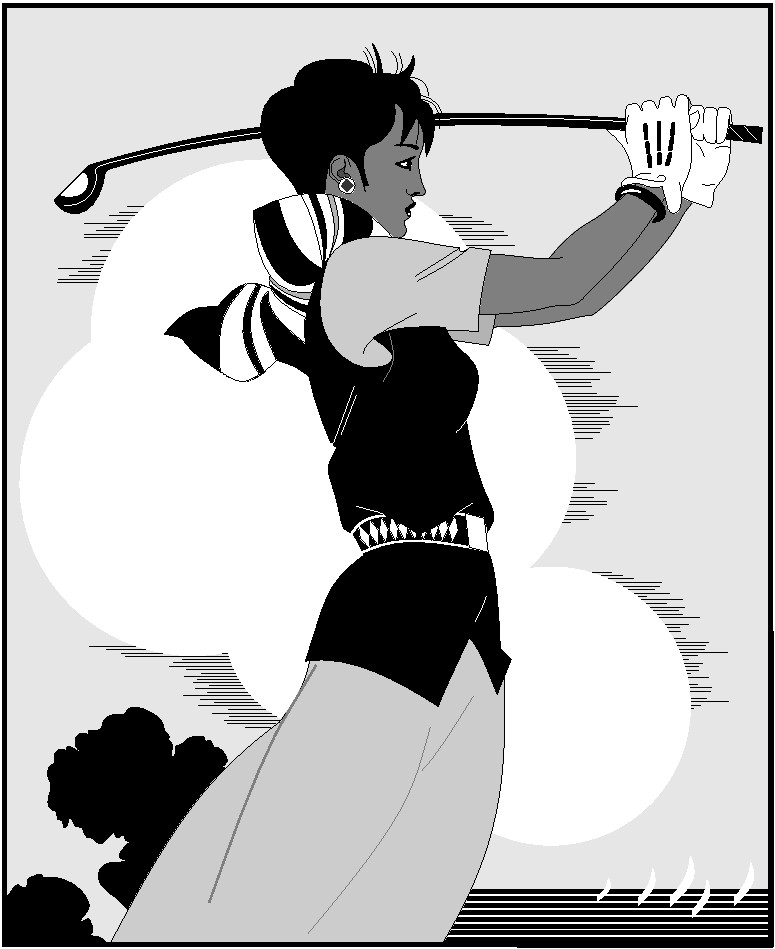
\includegraphics[width = 0.4\textwidth]{golfer}
  \bicaption[golfer1]{}{打高尔夫球球的人(博士论文双语题注)}{Fig.$\!$}{The person playing golf (Doctoral thesis)}
\end{figure}

\subsection{并排图和子图}[Abreast-picture and Sub-picture example]
\subsubsection{并排图}[Abreast-picture example]

使用并排图时,需要注意对齐方式。默认情况是中部对齐。这里给出中部对齐、顶部对齐
、图片底部对齐三种常见方式。其中,底部对齐方式有一个很巧妙的方式,将长度比较小
的图放在左面即可。

\begin{figure}[htbp]
  \centering
  \begin{minipage}{0.4\textwidth}
    \centering
    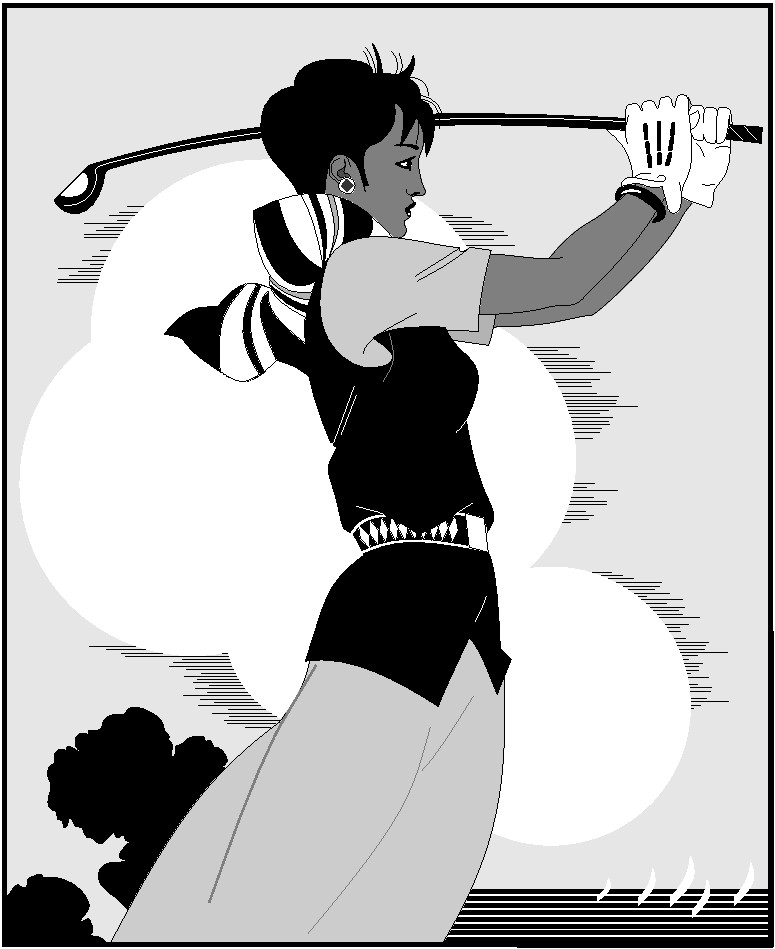
\includegraphics[width=\textwidth]{golfer}
    \bicaption[golfer2]{}{打高尔夫球的人}{Fig.$\!$}{The person playing golf}
  \end{minipage}
  \centering
  \begin{minipage}{0.4\textwidth}
    \centering
    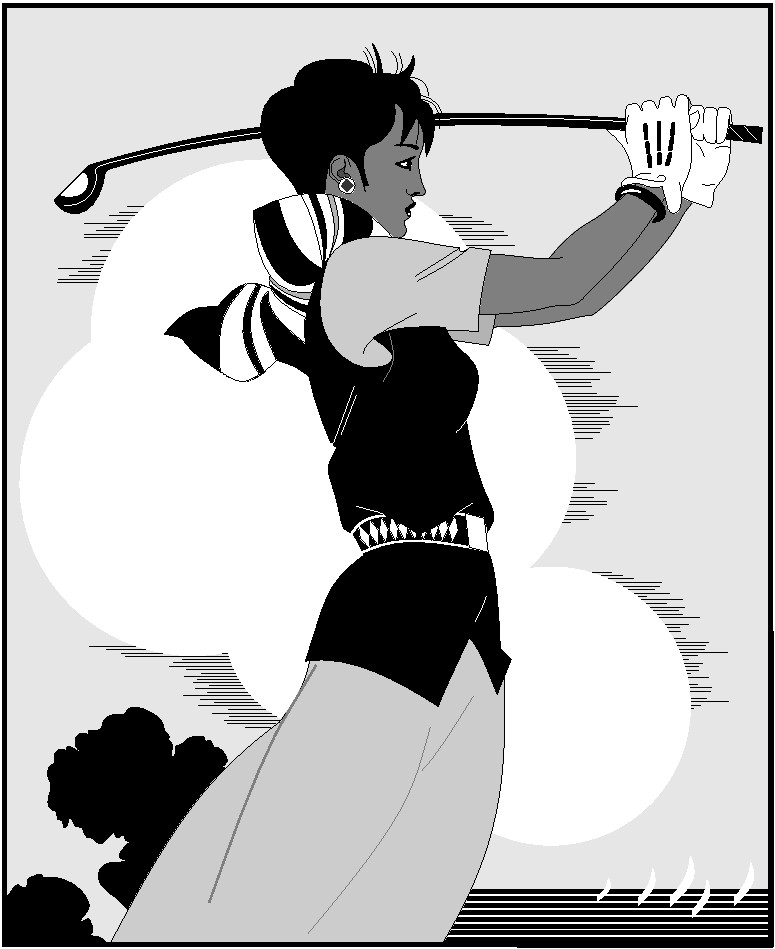
\includegraphics[width=\textwidth]{golfer}
    \bicaption[golfer3]{}{打高尔夫球的人。注意,这里默认居中}{Fig.$\!$}{The person playing golf. Please note that, it is vertically center aligned by default.}
  \end{minipage}
\end{figure}

\begin{figure}[htbp]
  \centering
  \begin{minipage}[t]{0.4\textwidth}
    \centering
    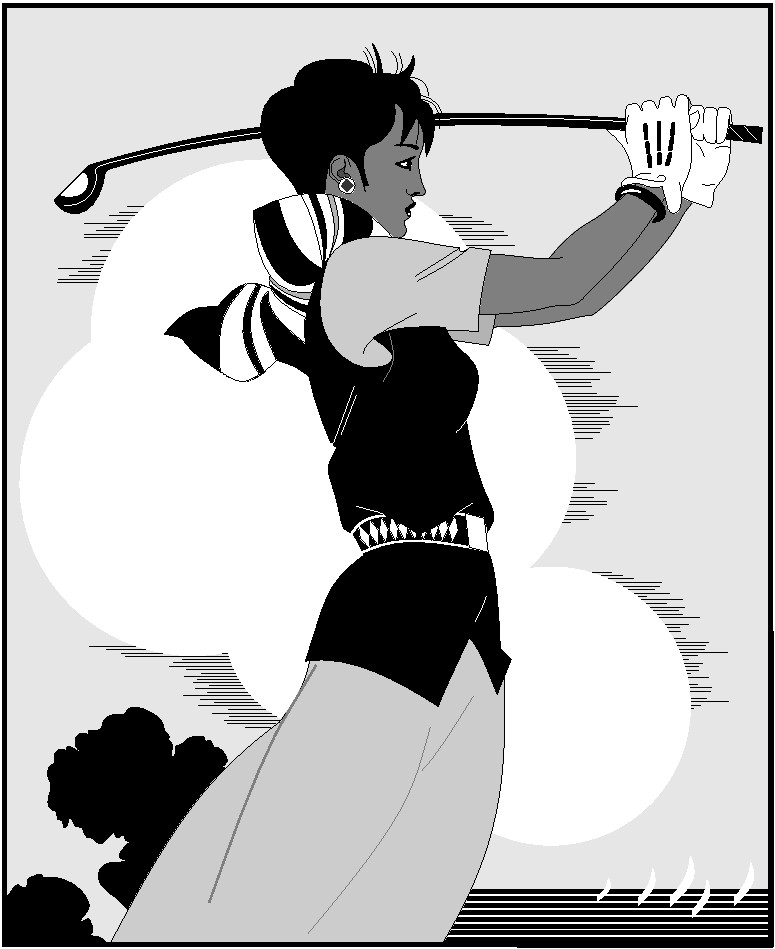
\includegraphics[width=\textwidth]{golfer}
    \bicaption[golfer5]{}{打高尔夫球的人}{Fig.$\!$}{The person playing golf}
  \end{minipage}
  \centering
  \begin{minipage}[t]{0.4\textwidth}
    \centering
    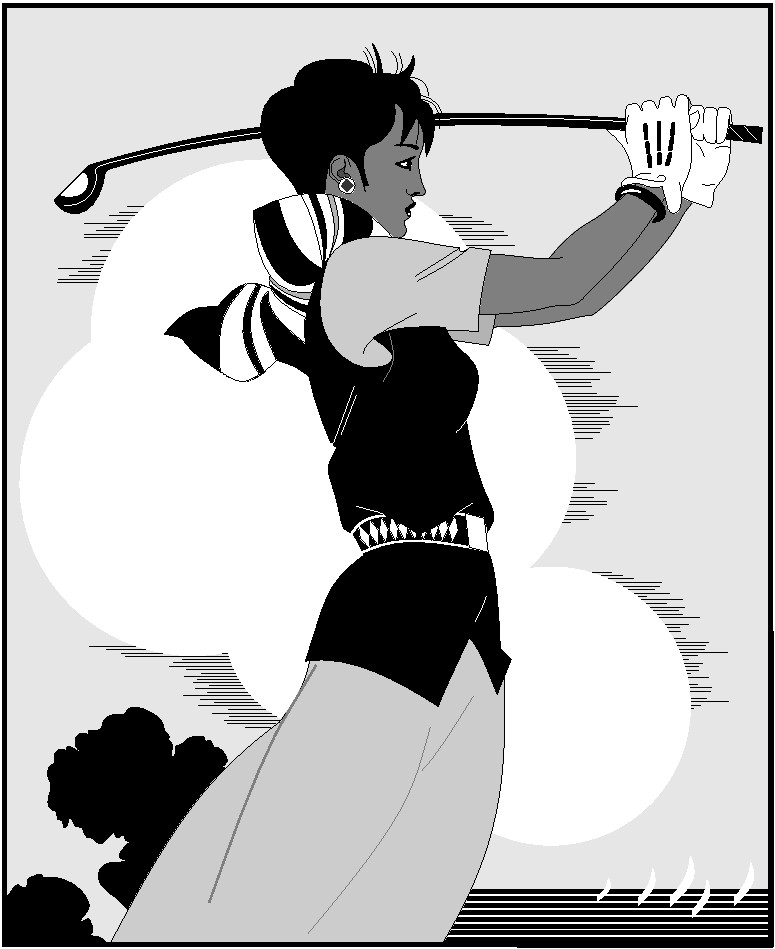
\includegraphics[width=\textwidth]{golfer}
    \bicaption[golfer8]{}{打高尔夫球的人。注意,此图是顶部对齐}{Fig.$\!$}{The person playing golf. Please note that, it is vertically top aligned.}
  \end{minipage}
\end{figure}

\begin{figure}[htbp]
  \centering
  \begin{minipage}[t]{0.4\textwidth}
    \centering
    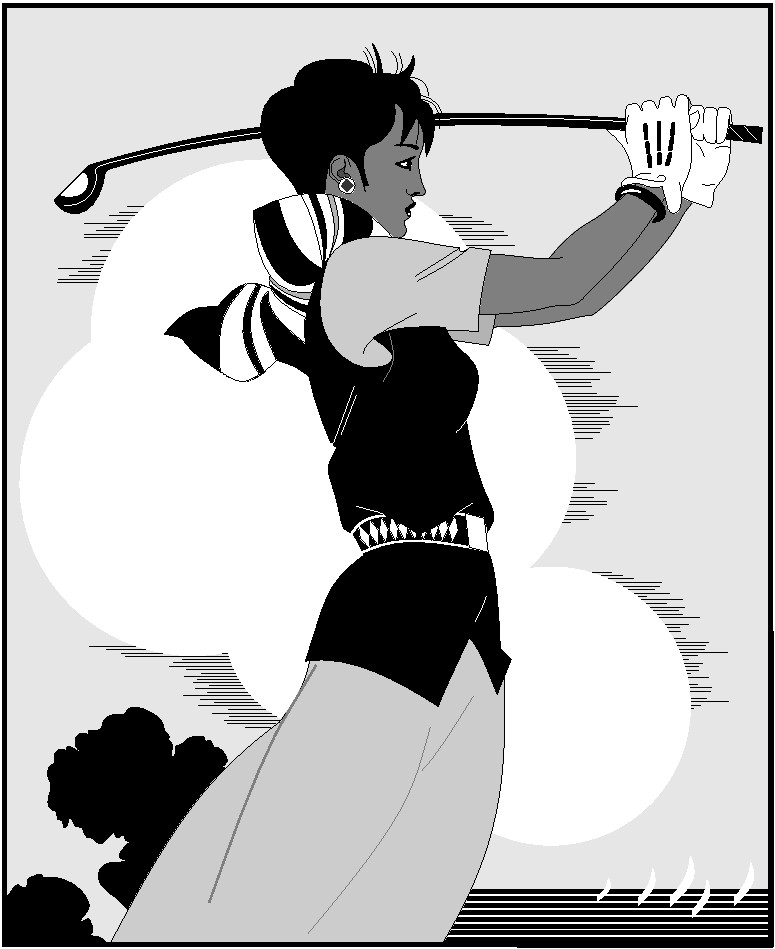
\includegraphics[width=\textwidth,height=\textwidth]{golfer}
    \bicaption[golfer9]{}{打高尔夫球的人。注意,此图对齐方式是图片底部对齐}{Fig.$\!$}{The person playing golf. Please note that, it is vertically bottom aligned for figure.}
  \end{minipage}
  \centering
  \begin{minipage}[t]{0.4\textwidth}
    \centering
    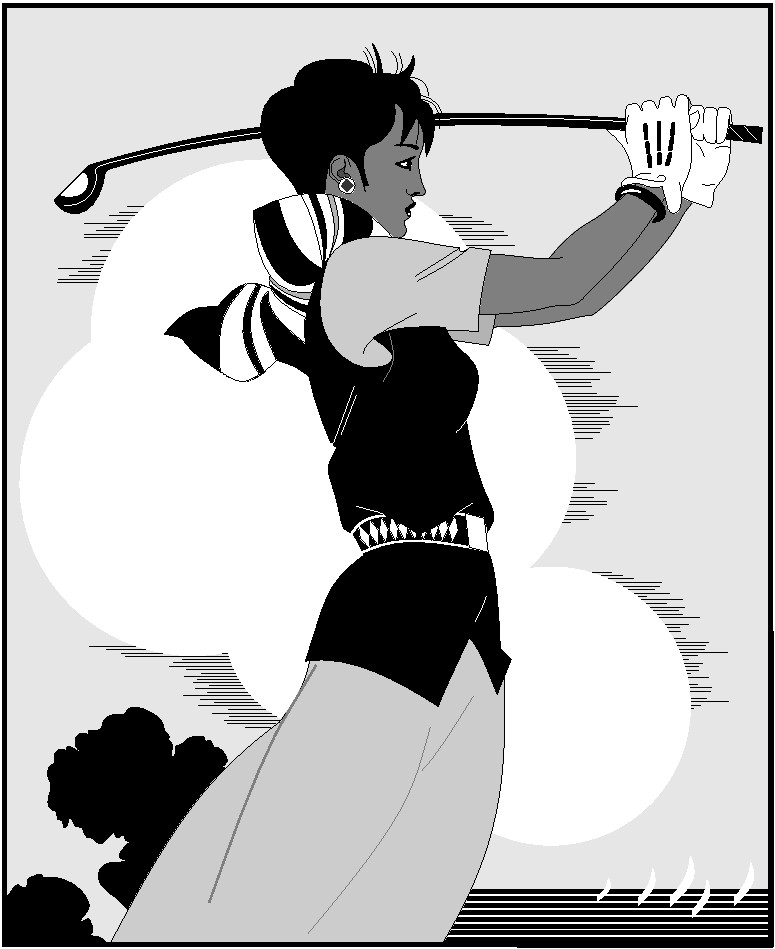
\includegraphics[width=\textwidth]{golfer}
    \bicaption[golfer6]{}{打高尔夫球的人}{Fig.$\!$}{The person playing golf}
  \end{minipage}
\end{figure}

\subsubsection{子图}[Sub-picture example]
注意:子图题注也可以只用中文。规范规定“分图题置于分图之下或图题之下”,但没有给出具体的格式要求。
没有要求的另外一个说法就是“无论什么格式都不对”。

所以只有在一个图中有标注“(a),(b)”,无法使用\cs{subfigure}的情况下,使用最后一个图例中的格式设置方法,否则不要使用。

子图图题使用“minipage”和“description”环境,宽度,对齐方式可以按照需要自由设置。

\begin{figure}[!h]
  \setlength{\subfigcapskip}{-1bp}
  \centering
  \begin{minipage}{\textwidth}
    \centering
    \subfigure{\label{golfer41}}\addtocounter{subfigure}{-2}
    \subfigure[The person playing golf]{\subfigure[打高尔夫球的人~1]{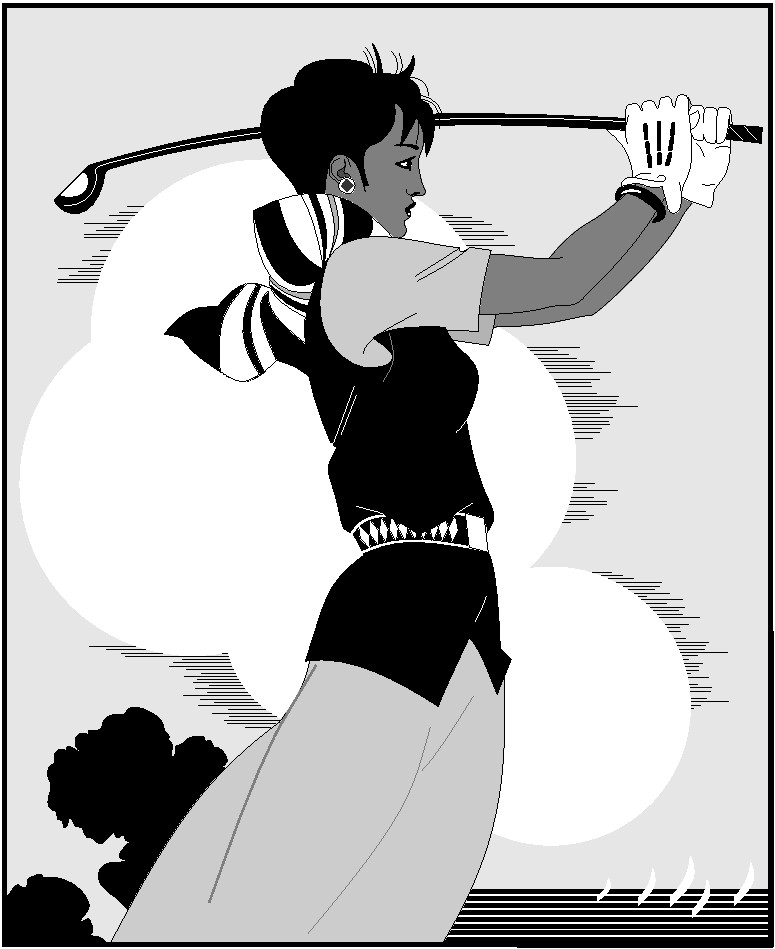
\includegraphics[width=0.4\textwidth]{golfer}}}
    \hspace{2em}
    \subfigure{\label{golfer42}}\addtocounter{subfigure}{-2}
    \subfigure[The person playing golf]{\subfigure[打高尔夫球的人~2]{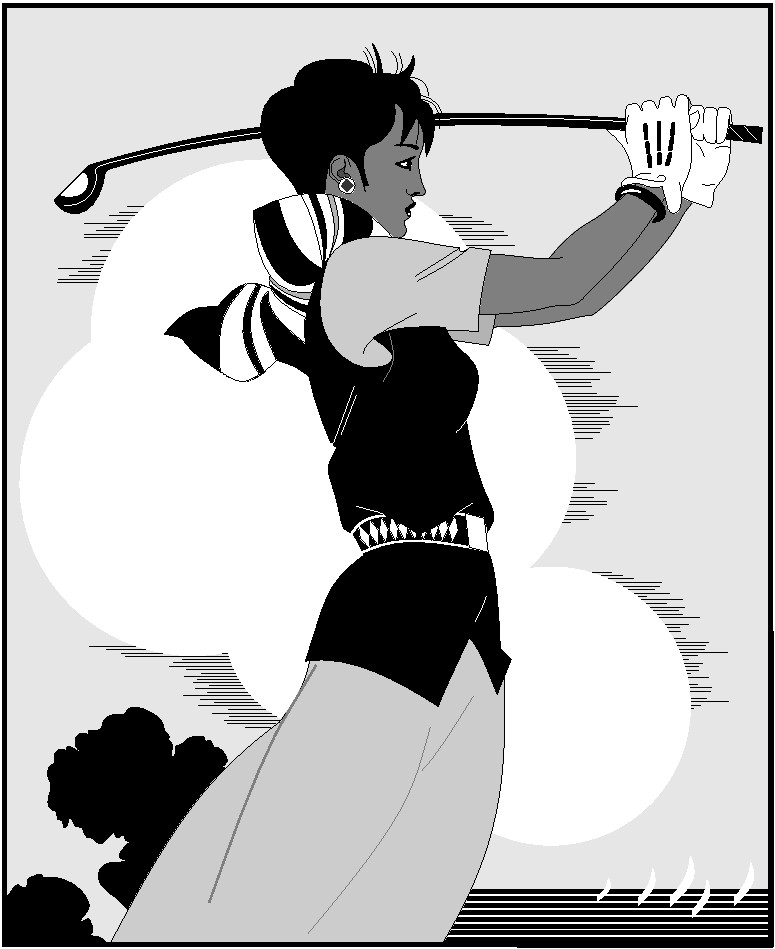
\includegraphics[width=0.4\textwidth]{golfer}}}
  \end{minipage}
  \centering
  \begin{minipage}{\textwidth}
    \centering
    \subfigure{\label{golfer43}}\addtocounter{subfigure}{-2}
    \subfigure[The person playing golf]{\subfigure[打高尔夫球的人~3]{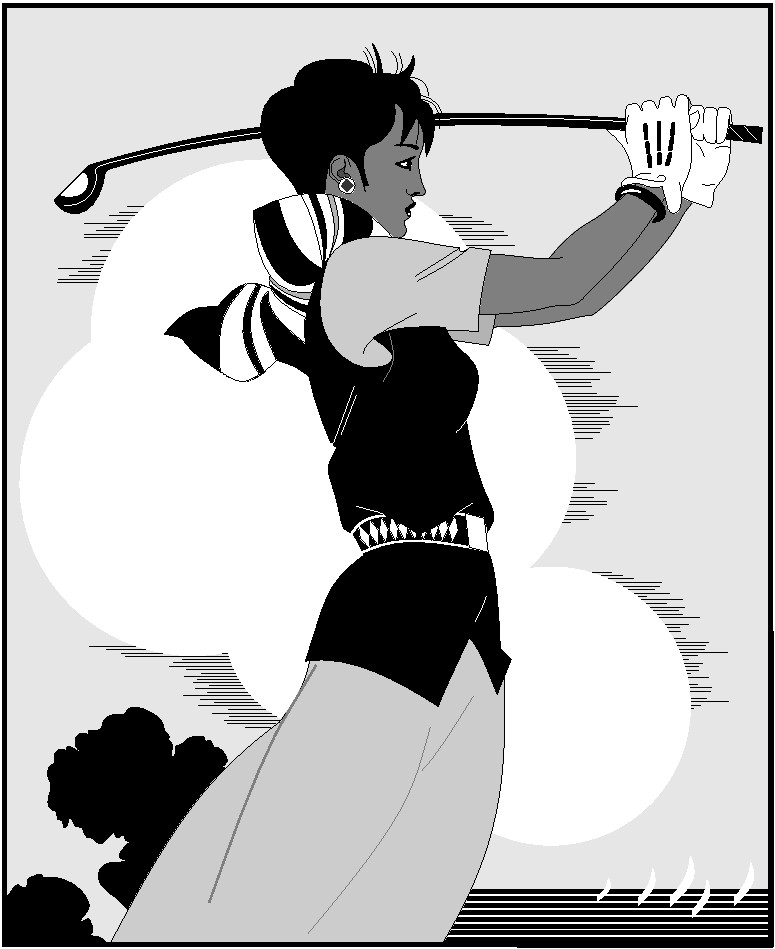
\includegraphics[width=0.4\textwidth]{golfer}}}
    \hspace{2em}
    \subfigure{\label{golfer44}}\addtocounter{subfigure}{-2}
    \subfigure[The person playing golf. Here, 'hang indent' and 'center last line' are not stipulated in the regulation.]{\subfigure[打高尔夫球的人~4。注意,规范中没有明确规定要悬挂缩进、最后一行居中。]{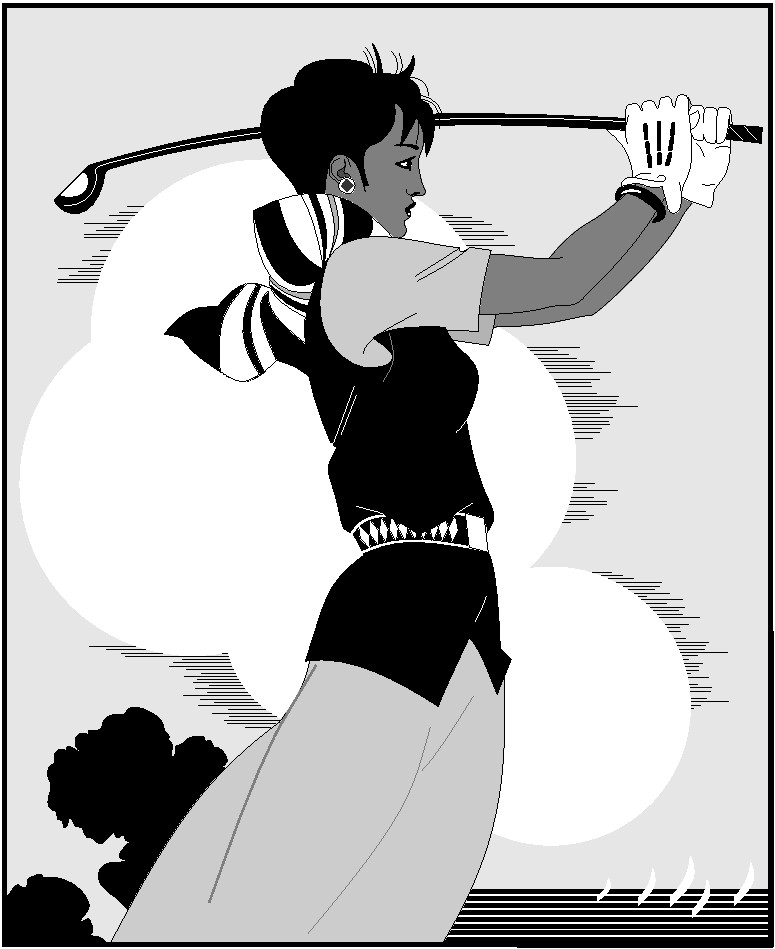
\includegraphics[width=0.4\textwidth]{golfer}}}
  \end{minipage}
  \vspace{0.2em}
  \bicaption[golfer4]{}{打高尔夫球的人}{Fig.$\!$}{The person playing gol}
\end{figure}

\begin{figure}[t]
  \centering
  \begin{minipage}{.7\linewidth}
    \setlength{\subfigcapskip}{-1bp}
    \centering
    \begin{minipage}{\textwidth}
      \centering
      \subfigure{\label{golfer45}}\addtocounter{subfigure}{-2}
      \subfigure[The person playing golf]{\subfigure[打高尔夫球的人~1]{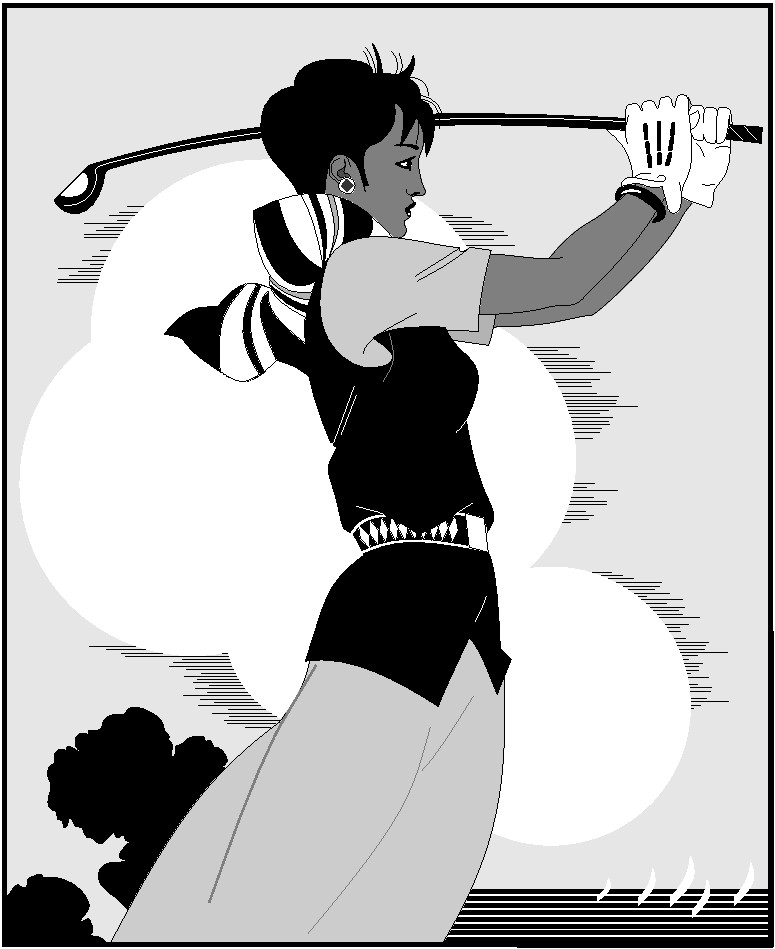
\includegraphics[width=0.4\textwidth]{golfer}}}
      \hspace{4em}
      \subfigure{\label{golfer46}}\addtocounter{subfigure}{-2}
      \subfigure[The person playing golf]{\subfigure[打高尔夫球的人~2]{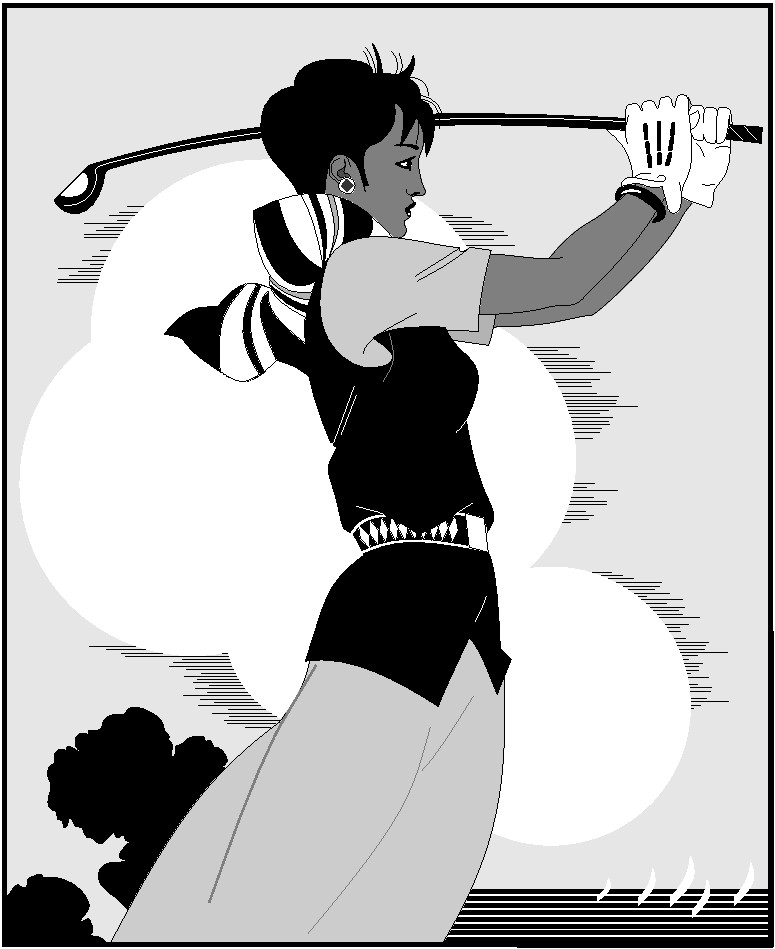
\includegraphics[width=0.4\textwidth]{golfer}}}
    \end{minipage}
    \vspace{0.2em}
    \bicaption[golfer47]{}{打高尔夫球的人}{Fig.$\!$}{The person playing golf.}
  \end{minipage}
\end{figure}

\begin{figure}[t]
  \centering
  \begin{tikzpicture}
    \node[anchor=south west,inner sep=0] (image) at (0,0) {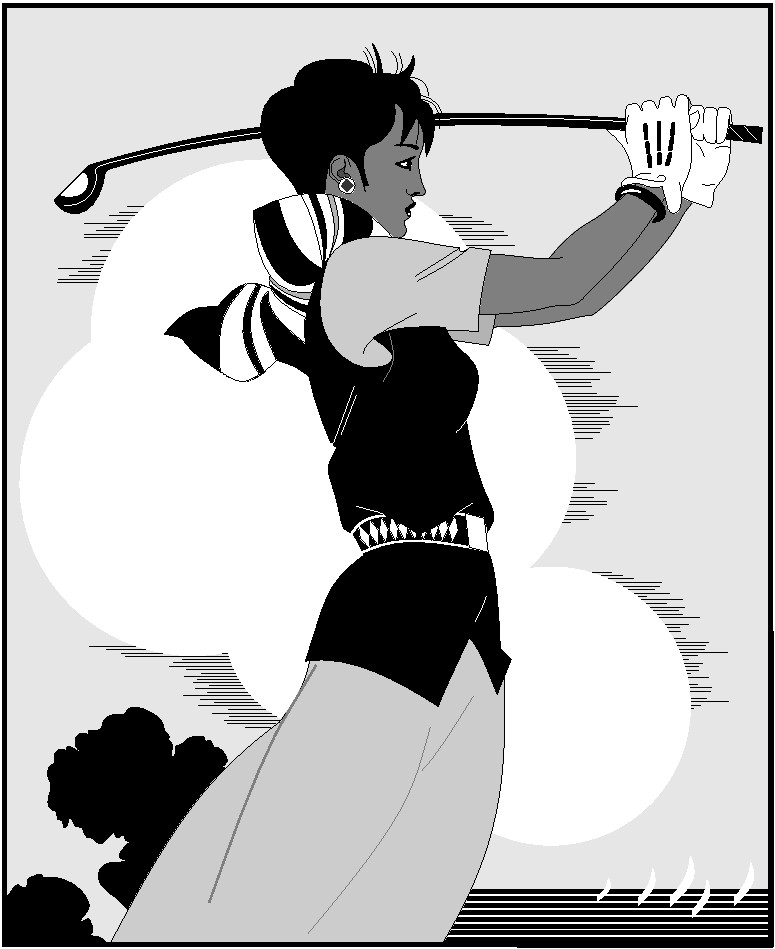
\includegraphics[width=0.3\textwidth]{golfer}};
    \begin{scope}[x={(image.south east)},y={(image.north west)}]
      \node at (0.3,0.5) {a)};
      \node at (0.8,0.2) {b)};
    \end{scope}
  \end{tikzpicture}
  \bicaption[golfer0]{}{打高尔夫球球的人(硕士论文双语题注)}{Fig.$\!$}{The person playing golf (Master thesis)}
  \vskip -0.4em
  \hspace{2em}
  \begin{minipage}[t]{0.3\textwidth}
    \wuhao \setlist[description]{font=\normalfont}
    \begin{description}
      \item[(a)]a点说明
    \end{description}
  \end{minipage}
  \hspace{2em}
  \begin{minipage}[t]{0.3\textwidth}
    \wuhao \setlist[description]{font=\normalfont}
    \begin{description}
      \item[(b)]b点说明
      \item[(b)]Note of Point b
    \end{description}
  \end{minipage}
\end{figure}


\begin{figure}[!h]
  \centering
  \begin{sideways}
    \begin{minipage}{\textheight}
      \centering
      \fbox{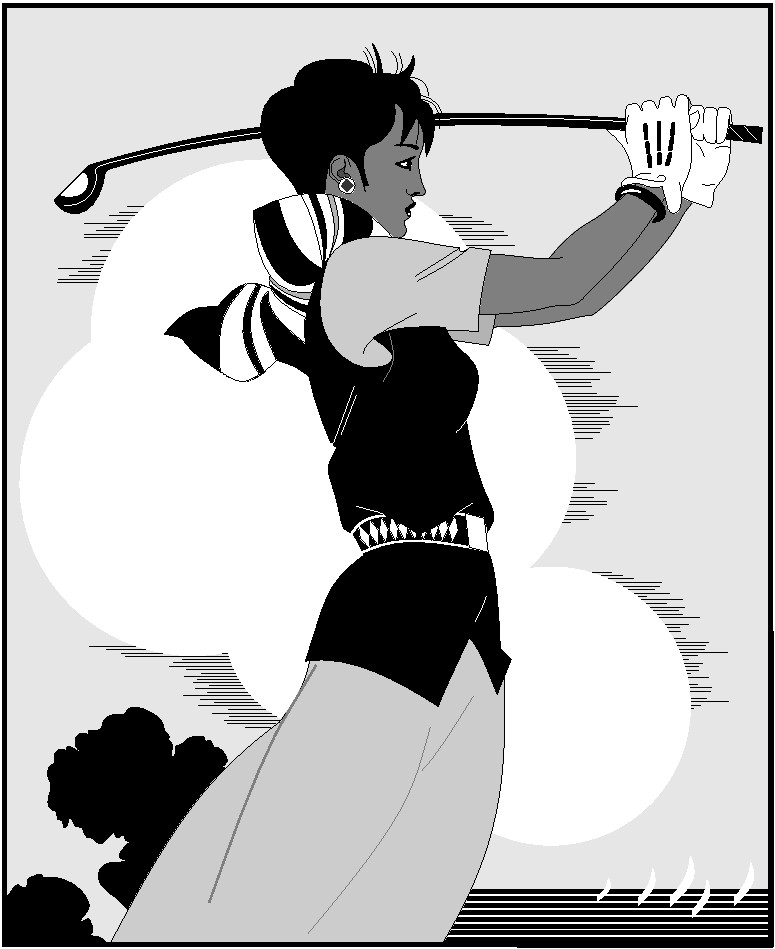
\includegraphics[width=0.2\textwidth]{golfer}}
      \fbox{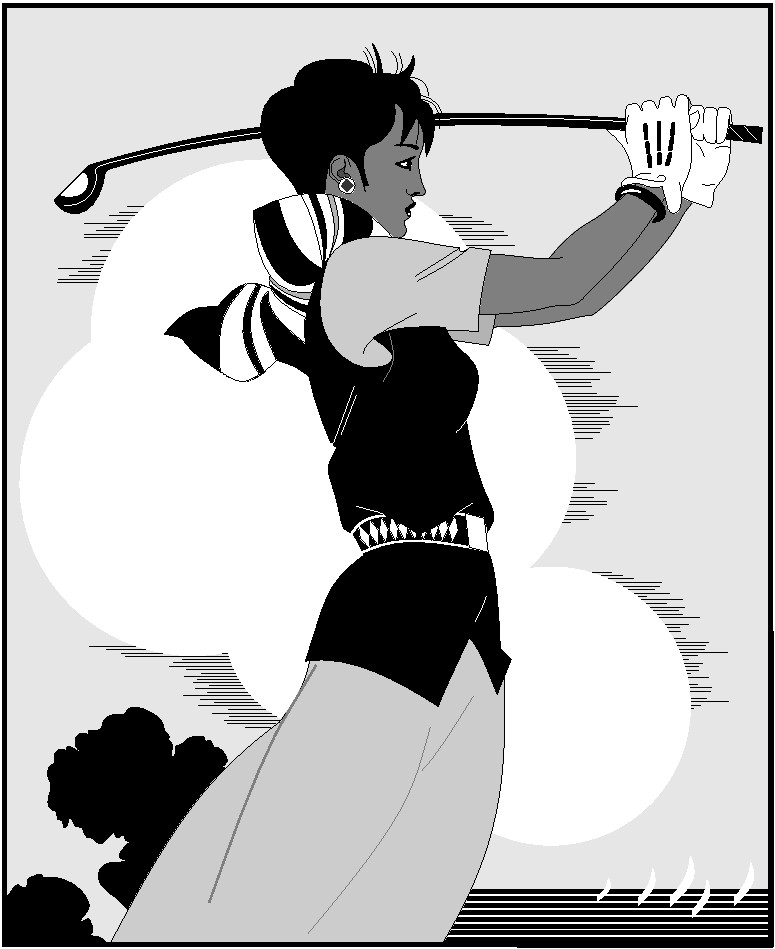
\includegraphics[width=0.2\textwidth]{golfer}}
      \fbox{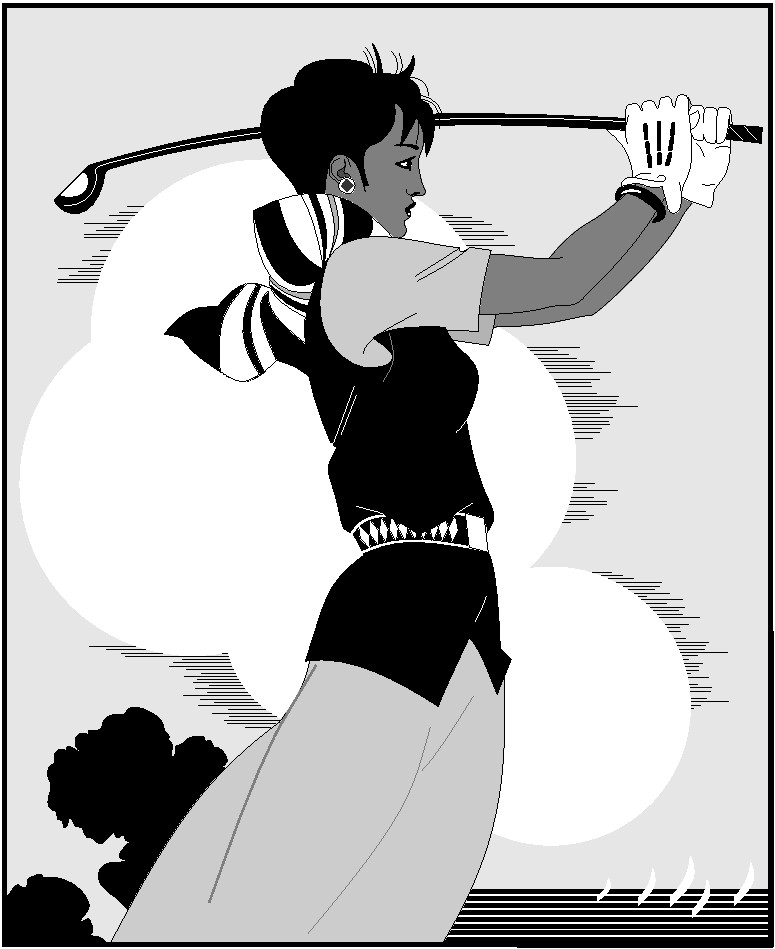
\includegraphics[width=0.2\textwidth]{golfer}}
      \fbox{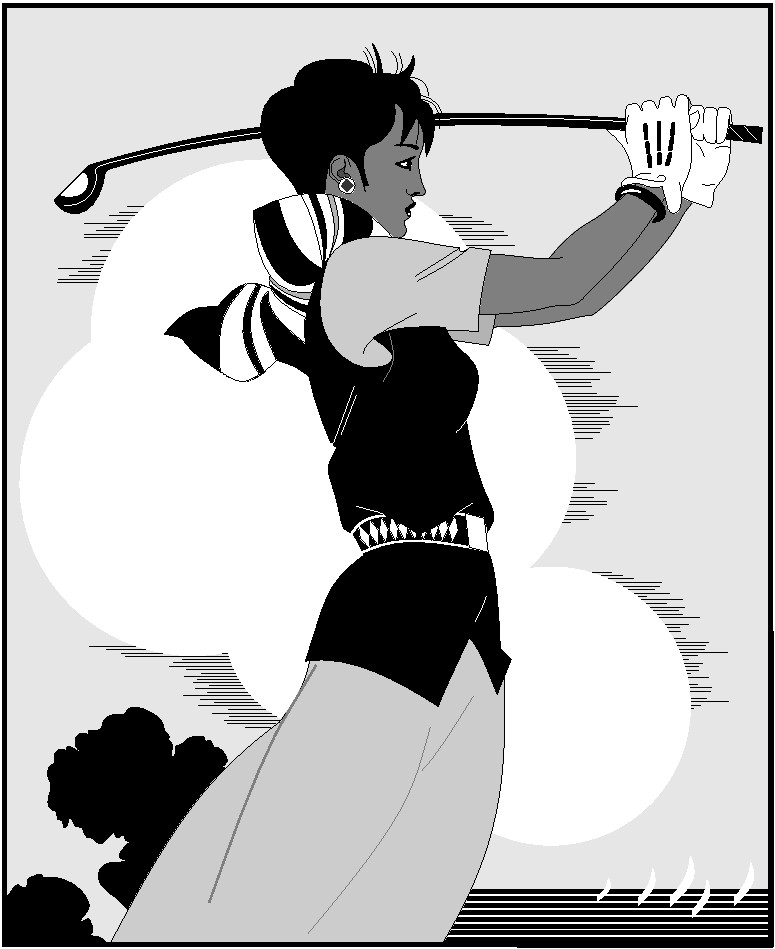
\includegraphics[width=0.2\textwidth]{golfer}}
      \fbox{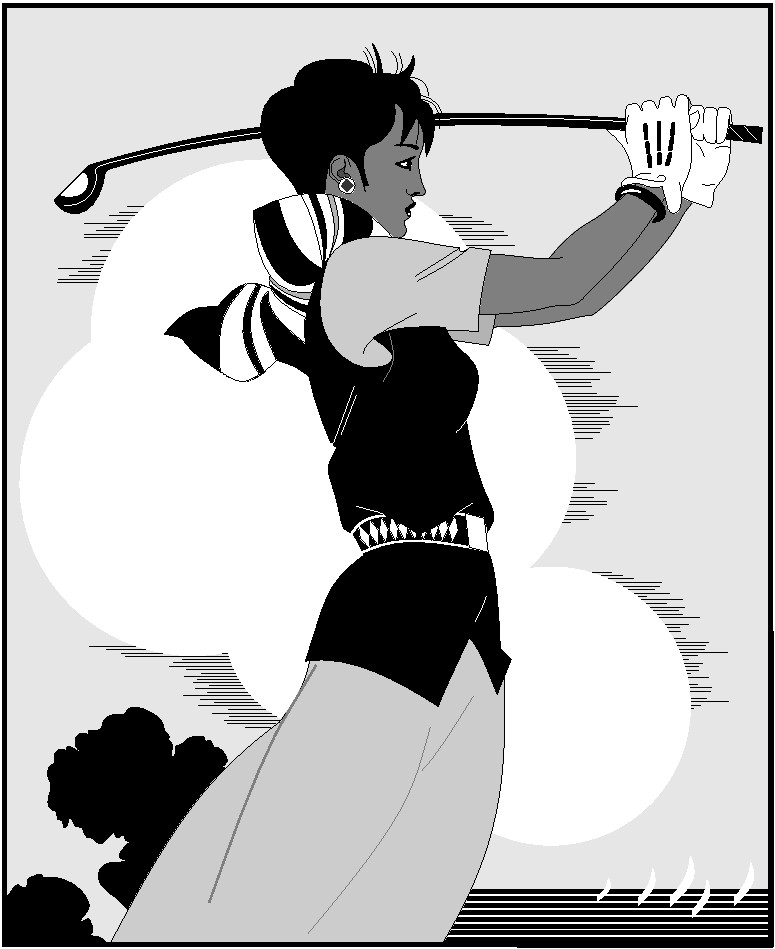
\includegraphics[width=0.2\textwidth]{golfer}}
      \fbox{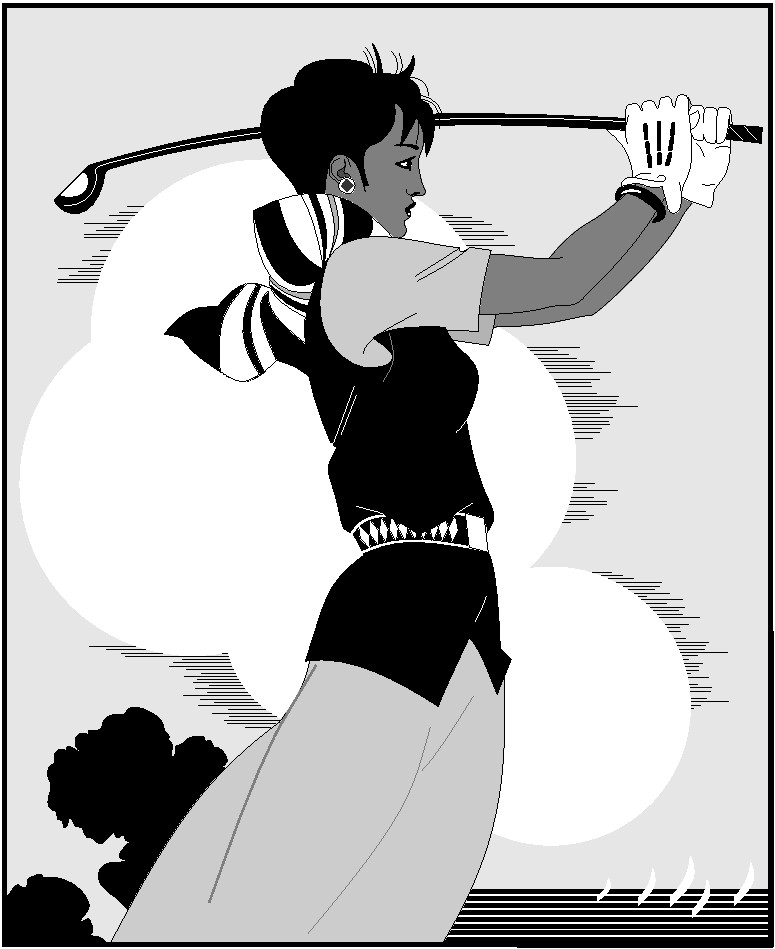
\includegraphics[width=0.2\textwidth]{golfer}}
      \fbox{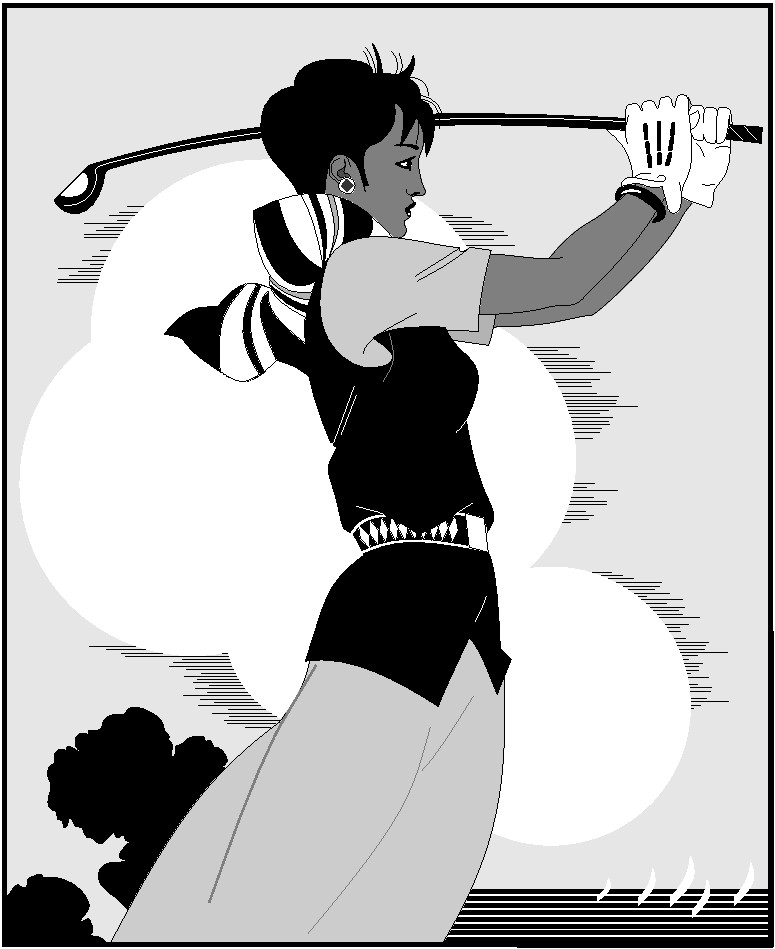
\includegraphics[width=0.2\textwidth]{golfer}}
      \bicaption[golfer7]{}{打高尔夫球的人(多图组合)}{Fig.$\!$}{The person playing golf (Many pictures arrange)}
    \end{minipage}
  \end{sideways}
\end{figure}

\clearpage

如果不想让图片浮动到下一章节,那么在此处使用\cs{clearpage}命令。

\section{如何做出符合规范的漂亮的图}
关于作图工具在后文~\ref{drawtool}~中给出一些作图工具的介绍,此处不多介绍。

此处以Tikz为例说明如何做出符合规范的图。

\subsection{Tikz作图举例}
使用Tikz作图核心思想是把格式、主题、样式与内容分离,定义在全局中。

注意字体设置可以有两种选择,如何字少,用五号字,字多用小五。

使用Tikz作图不会出现字体问题,字体会自动与正文一致。

\begin{figure}[thb!]
  \centering
  \begin{tikzpicture}[xscale=0.8,yscale=0.3,rotate=90]
    \small
    \draw (-22,6.5) node[refcell]{参考基因组};
    \draw[refline] (-23, 5) -- (27, 5);
    \draw (-22,3.75) node[tscell]{肿瘤样本};
    \draw (-20,3.75) node[tncell]{正常细胞};
    \draw[tnline] (-21, 2.5) -- (27, 2.5);
    \draw (-20,1.25) node[ttcell]{肿瘤细胞};
    \rcell{2}{6};
    \draw[fakeevolve] (4.5, 5.25) -- (4.5, 4.8);
    \ncell{2}{4};
    \draw[evolve] (4.5, 3) .. controls (4.5,2.8) and (-3.5,2.9) ..  (-3.5, 2);
    \draw[evolve] (4.5, 3) .. controls (4.5,2.8) and (11.5,2.9) .. (11.5, 2);
    \tcellone{-6}{1.5};
    \draw (-9, 2) node[ttcell]{1};
    \draw[evolve] (-3.5, 0) .. controls (-3.5,-0.2) and (-12,-0.1) .. (-12, -1.5);
    \draw[evolve] (-3.5, 0) .. controls (-3.5,-0.2) and (1.5,-0.1) .. (1.5, -1.5);
    \tcellthree{7}{1.5};
    \draw (4, 2) node[ttcell]{2};
    \draw[evolve] (11, 0.5) .. controls (11,0.3) and (19,0.4) .. (19, -1.5);
    \tcellfive{-16}{-2};
    \draw (-19, -1.5) node[ttcell]{3};
    \tcelltwo{-1}{-2};
    \draw (-4, -1.5) node[ttcell]{4};
    \tcellfour{12}{-2};
    \draw (9, -1.5) node[ttcell]{5};
  \end{tikzpicture}
  \begin{minipage}{.9\linewidth}
    \vskip 0.2em
    \wuhao 图中,带有箭头的淡蓝色箭头表示肿瘤子种群的进化方向。一般地,从肿瘤组织中取用于进行二代测序的样本中含有一定程度的正常细胞污染,因此肿瘤的样本中含有正常细胞和肿瘤细胞。每一个子种群的基因组的模拟过程是把生殖细胞变异和体细胞变异加入到参考基因组中。
    \vspace{0.6em}
  \end{minipage}
  \bicaption[tumor]{}{肿瘤组织中各个子种群的进化示意图}{Fig.$\!$}{The diagram of tumor subpopulation evolution process}
\end{figure}

\section{表格}

表应有自明性。表格不加左、右边线。表的编排建议采用国际通行的三线表。表中文字用宋
体~5~号字。每个表格均应有表题(由表序和表名组成)。表序一般按章编排,如第~1~章第
一个插表的序号为“表~1.1”等。表序与表名之间空一格,表名中不允许使用标点符号,表名
后不加标点。表题置于表上,硕士学位论文只用中文,博士学位论文用中、英文两种文字居
中排写,中文在上,要求中文用宋体~5~号字,英文用新罗马字体~5~号字。表头设计应简单
明了,尽量不用斜线。表头中可采用化学符号或物理量符号。


\subsection{普通表格的绘制方法}[Methods of drawing normal tables]

表格应具有三线表格式,因此需要调用~booktabs~宏包,其标准格式如表~\ref{table1}~所示。
\begin{table}[htbp]
  \bicaption[table1]{}{符合研究生院绘图规范的表格}{Table$\!$}{Table in agreement of the standard from graduate school}
  \vspace{0.5em}\centering\wuhao
  \begin{tabular}{ccccc}
    \toprule[1.5pt]
    $D$(in) & $P_u$(lbs) & $u_u$(in) & $\beta$ & $G_f$(psi.in) \\
    \midrule[1pt]
    5       & 269.8      & 0.000674  & 1.79    & 0.04089       \\
    10      & 421.0      & 0.001035  & 3.59    & 0.04089       \\
    20      & 640.2      & 0.001565  & 7.18    & 0.04089       \\
    \bottomrule[1.5pt]
  \end{tabular}
\end{table}
全表如用同一单位,则将单位符号移至表头右上角,加圆括号。表中数据应准确无误,书写
清楚。数字空缺的格内加横线“-”(占~2~个数字宽度)。表内文字或数字上、下或左、右
相同时,采用通栏处理方式,不允许用“〃”、“同上”之类的写法。表内文字说明,起行空一
格、转行顶格、句末不加标点。如某个表需要转页接排,在随后的各页上应重复表的编号。
编号后加“(续表)”,表题可省略。续表应重复表头。

\subsection{列宽可调表格的绘制方法}[Methods of drawing tables with adjustable-width columns]
论文中能用到列宽可调表格的情况共有两种,一种是当插入的表格某一单元格内容过长以至
于一行放不下的情况,另一种是当对公式中首次出现的物理量符号进行注释的情况,这两种
情况都需要调用~tabularx~宏包。下面将分别对这两种情况下可调表格的绘制方法进行阐述
。
\subsubsection{表格内某单元格内容过长的情况}[The condition when the contents in
  some cells of tables are too long]
首先给出这种情况下的一个例子如表~\ref{table3}~所示。
\begin{table}[htbp]
  \centering
  \bicaption[table3]{}{最小的三个正整数的英文表示法}{Table$\!$}{The English construction of the smallest three positive integral numbers}\vspace{0.5em}\wuhao
  \begin{tabularx}{0.7\textwidth}{llX}
    \toprule[1.5pt]
    Value & Name  & Alternate names, and names for sets of the given size                                                                                           \\\midrule[1pt]
    1     & One   & ace, single, singleton, unary, unit, unity                                                                                                      \\
    2     & Two   & binary, brace, couple, couplet, distich, deuce, double, doubleton, duad, duality, duet, duo, dyad, pair, snake eyes, span, twain, twosome, yoke \\
    3     & Three & deuce-ace, leash, set, tercet, ternary, ternion, terzetto, threesome, tierce, trey, triad, trine, trinity, trio, triplet, troika, hat-trick     \\\bottomrule[1.5pt]
  \end{tabularx}
\end{table}
tabularx环境共有两个必选参数:第1个参数用来确定表格的总宽度,第2个参数用来确定每
列格式,其中标为X的项表示该列的宽度可调,其宽度值由表格总宽度确定。标为X的列一般
选为单元格内容过长而无法置于一行的列,这样使得该列内容能够根据表格总宽度自动分行
。若列格式中存在不止一个X项,则这些标为X的列的列宽相同,因此,一般不将内容较短的
列设为X。标为X的列均为左对齐,因此其余列一般选为l(左对齐),这样可使得表格美观
,但也可以选为c或r。

\subsubsection{对物理量符号进行注释的情况}[The condition when physical symbols
  need to be annotated]

为使得对公式中物理量符号注释的转行与破折号“——”后第一个字对齐,此处最好采用表格
环境。此表格无任何线条,左对齐,且在破折号处对齐,一共有“式中”二字、物理量符号和
注释三列,表格的总宽度可选为文本宽度,因此应该采用\verb|tabularx|环境。由
\verb|tabularx|环境生成的对公式中物理量符号进行注释的公式如式(\ref{eq:1})所示。
\begin{equation}\label{eq:1}
  \ddot{\boldsymbol{\rho}}-\frac{\mu}{R_{t}^{3}}\left(3\mathbf{R_{t}}\frac{\mathbf{R_{t}\rho}}{R_{t}^{2}}-\boldsymbol{\rho}\right)=\mathbf{a}
\end{equation}
\begin{tabularx}{\textwidth}{@{}l@{\quad}r@{——}X@{}}
  式中 & $\boldsymbol{\rho}$        & 追踪飞行器与目标飞行器之间的相对位置矢量; \\
       & $\boldsymbol{\ddot{\rho}}$ & 追踪飞行器与目标飞行器之间的相对加速度;   \\
       & $\mathbf{a}$               & 推力所产生的加速度;                       \\
       & $\mathbf{R_t}$             & 目标飞行器在惯性坐标系中的位置矢量;       \\
       & $\omega_{t}$               & 目标飞行器的轨道角速度;                   \\
       & $\mathbf{g}$               & 重力加速度,$=\frac{\mu}{R_{t}^{3}}\left(
    3\mathbf{R_{t}}\frac{\mathbf{R_{t}\rho}}{R_{t}^{2}}-\boldsymbol{\rho}\right)=\omega_{t}^{2}\frac{R_{t}}{p}\left(
    3\mathbf{R_{t}}\frac{\mathbf{R_{t}\rho}}{R_{t}^{2}}-\boldsymbol{\rho}\right)$,这里~$p$~是目标飞行器的轨道半通径。
\end{tabularx}\vspace{3.15bp}
由此方法生成的注释内容应紧邻待注释公式并置于其下方,因此不能将代码放入
\verb|table|浮动环境中。但此方法不能实现自动转页接排,可能会在当前页剩余空间不够
时,全部移动到下一页而导致当前页出现很大空白。因此在需要转页处理时,还请您手动将
需要转页的代码放入一个新的\verb|tabularx|环境中,将原来的一个\verb|tabularx|环境
拆分为两个\verb|tabularx|环境。

\subsubsection{排版横版表格的举例}[An example of landscape table]
由于版面设置方向调整,使用横版排版的表格必须另起一页,例如表~\ref{table4}。

\begin{table}[p]
  \centering
  \begin{sideways}
    \begin{minipage}{\textheight}
      \bicaption[table4]{}{不在规范中规定的横版表格}{Table$\!$}{A table style which is not stated in the regulation}
      \vspace{0.5em}\centering\wuhao
      \begin{tabular}{ccccc}
        \toprule[1.5pt]
        $D$(in) & $P_u$(lbs) & $u_u$(in) & $\beta$ & $G_f$(psi.in) \\
        \midrule[1pt]
        5       & 269.8      & 0.000674  & 1.79    & 0.04089       \\
        10      & 421.0      & 0.001035  & 3.59    & 0.04089       \\
        20      & 640.2      & 0.001565  & 7.18    & 0.04089       \\
        \bottomrule[1.5pt]
      \end{tabular}
    \end{minipage}
  \end{sideways}
\end{table}


\section{公式}
与正常\LaTeX\ 使用方法一致,此处略。关于公式中符号样式的定义在`heuthesis.sty'有示例。

\section{其他杂项}[Miscellaneous]

\subsection{右翻页}[Open right]

对于双面打印的论文,强制使每章的标题页出现右手边为右翻页。
规范中没有明确规定是否是右翻页打印。
模板给出了右翻页选项。
为了应对用户的个人喜好,在希望设置成右翻页的位置之前添加\cs{cleardoublepage}命令即可。

\subsection{算法}[Algorithms]
我校算法有以下几大特点。

(1)算法不在规范中要求。

(2)算法常常被使用(至少计算机学院)。

(3)格式乱,甚至出现了每个实验室的格式要求都不一样。

此处不给出示例,因为没法给。

\subsection{脚注}[Footnotes]
不在再规范\footnote{规范是指\PGR\ 和\UGR}中要求,模板默认使用清华大学的格式。

\subsection{源码}[Source code]
也不在再规范中要求。如果有需要可以使用lstlisting环境。

\begin{lstlisting}[flexiblecolumns,numbers=left,language={[ANSI]C}]
    int main(int argc, char ** argv)
    {
        printf("`我爱中文`!\n");
        return 0;
    }
\end{lstlisting}

\subsection{专业绘图工具}[Processional drawing tool]
\label{drawtool}
推荐使用tikz包,使用tikz源码绘图的好处是,图片中的字体与正文中的字体一致。具体如
何使用tikz绘图不属于模板范畴。

tikz适合用来画不需要大量实验数据支撑示意图。但R语言等专业绘图工具具有画出各种、
专业、复杂的数据图。R语言中有tikz包,能自动生成tikz码,这样tikz几乎无所不能。
对于排版有极致追求的小伙伴,可以参考
\href{http://www.texample.net/tikz/resources/}{http://www.texample.net/tikz/resources/}
中所列工具,几乎所有作图软件所作的图形都可转成tikz,然后可以自由的在tikz中修改
图中内容,定义字体等等。实现前文我校规范中要求的图中字体的一致性的终极目标。


\subsection{术语词汇管理}[Manage glossaries]
推荐使用glossaries包管理术语、缩略语,可以自动生成首次全写,非首次缩写。

\subsection{\TeX\ 源码编辑器}[\TeX editor]
推荐:(1)付费软件Winedt;(2)免费软件TexStudio;(3)vim、vscodes或其他文本编辑器(需要配置)。

\subsection{\LaTeX\ 排版重要原则}[\LaTeX\ typesetting rules]
格式和内容分离是\LaTeX\ 最大优势,所有多次出现的内容、样式等等都可以定义为简单命
令、环境。这样的好处是方便修改、管理。例如,如果想要把所有的表示向量的符号由粗体
\cs{mathbf}变换到花体\cs{mathcal},只需修改该格式的命令的定义部分,不需要像MS
word那样处处修改。总而言之,使用自定义命令和环境才是正确的使用\LaTeX\ 的方式。


% Local Variables:
% TeX-master: "../main"
% TeX-engine: xetex
% End:


\backmatter
% !Mode:: "TeX:UTF-8" 
\begin{conclusions}

学位论文的结论作为论文正文的最后一章单独排写,但不加章标题序号。

结论应是作者在学位论文研究过程中所取得的创新性成果的概要总结,不能与摘要混为一谈。博士学位论文结论应包括论文的主要结果、创新点、展望三部分,在结论中应概括论文的核心观点,明确、客观地指出本研究内容的创新性成果(含新见解、新观点、方法创新、技术创新、理论创新),并指出今后进一步在本研究方向进行研究工作的展望与设想。对所取得的创新性成果应注意从定性和定量两方面给出科学、准确的评价,分(1)、(2)、(3)…条列出,宜用“提出了”、“建立了”等词叙述。

结论应是作者在学位论文研究过程中所取得的创新性成果的概要总结,不能与摘要混为一谈。博士学位论文结论应包括论文的主要结果、创新点、展望三部分,在结论中应概括论文的核心观点,明确、客观地指出本研究内容的创新性成果(含新见解、新观点、方法创新、技术创新、理论创新),并指出今后进一步在本研究方向进行研究工作的展望与设想。对所取得的创新性成果应注意从定性和定量两方面给出科学、准确的评价,分(1)、(2)、(3)…条列出,宜用“提出了”、“建立了”等词叙述。

结论应是作者在学位论文研究过程中所取得的创新性成果的概要总结,不能与摘要混为一谈。博士学位论文结论应包括论文的主要结果、创新点、展望三部分,在结论中应概括论文的核心观点,明确、客观地指出本研究内容的创新性成果(含新见解、新观点、方法创新、技术创新、理论创新),并指出今后进一步在本研究方向进行研究工作的展望与设想。对所取得的创新性成果应注意从定性和定量两方面给出科学、准确的评价,分(1)、(2)、(3)…条列出,宜用“提出了”、“建立了”等词叙述。

结论应是作者在学位论文研究过程中所取得的创新性成果的概要总结,不能与摘要混为一谈。博士学位论文结论应包括论文的主要结果、创新点、展望三部分,在结论中应概括论文的核心观点,明确、客观地指出本研究内容的创新性成果(含新见解、新观点、方法创新、技术创新、理论创新),并指出今后进一步在本研究方向进行研究工作的展望与设想。对所取得的创新性成果应注意从定性和定量两方面给出科学、准确的评价,分(1)、(2)、(3)…条列出,宜用“提出了”、“建立了”等词叙述。

结论应是作者在学位论文研究过程中所取得的创新性成果的概要总结,不能与摘要混为一谈。博士学位论文结论应包括论文的主要结果、创新点、展望三部分,在结论中应概括论文的核心观点,明确、客观地指出本研究内容的创新性成果(含新见解、新观点、方法创新、技术创新、理论创新),并指出今后进一步在本研究方向进行研究工作的展望与设想。对所取得的创新性成果应注意从定性和定量两方面给出科学、准确的评价,分(1)、(2)、(3)…条列出,宜用“提出了”、“建立了”等词叙述。

结论应是作者在学位论文研究过程中所取得的创新性成果的概要总结,不能与摘要混为一谈。博士学位论文结论应包括论文的主要结果、创新点、展望三部分,在结论中应概括论文的核心观点,明确、客观地指出本研究内容的创新性成果(含新见解、新观点、方法创新、技术创新、理论创新),并指出今后进一步在本研究方向进行研究工作的展望与设想。对所取得的创新性成果应注意从定性和定量两方面给出科学、准确的评价,分(1)、(2)、(3)…条列出,宜用“提出了”、“建立了”等词叙述。

结论应是作者在学位论文研究过程中所取得的创新性成果的概要总结,不能与摘要混为一谈。博士学位论文结论应包括论文的主要结果、创新点、展望三部分,在结论中应概括论文的核心观点,明确、客观地指出本研究内容的创新性成果(含新见解、新观点、方法创新、技术创新、理论创新),并指出今后进一步在本研究方向进行研究工作的展望与设想。对所取得的创新性成果应注意从定性和定量两方面给出科学、准确的评价,分(1)、(2)、(3)…条列出,宜用“提出了”、“建立了”等词叙述。

\end{conclusions}
   % 结论

\bibliographystyle{gbt7714-numerical}
\bibliography{reference}

% !Mode:: "TeX:UTF-8"
\begin{acknowledgements}
衷心感谢导师~XXX~教授对本人的精心指导。他的言传身教将使我终生受益。

……

感谢哈工大\LaTeX\ 论文模板\hithesis\ !

\end{acknowledgements}
 %致谢

% !Mode:: "TeX:UTF-8" 
\begin{publication}
\noindent\textbf{发表的相关论文}
\begin{publist}
\item XXX,XXX. Static Oxidation Model of Al-Mg/C Dissipation Thermal Protection Materials[J]. Rare Metal Materials and Engineering, 2010, 39(Suppl. 1): 520-524.(SCI~收录,IDS号为~669JS,IF=0.16)
\item XXX,XXX. 精密超声振动切削单晶铜的计算机仿真研究[J]. 系统仿真学报,2007,19(4):738-741,753.(EI~收录号:20071310514841)
\item XXX,XXX. 局部多孔质气体静压轴向轴承静态特性的数值求解[J]. 摩擦学学报,2007(1):68-72.(EI~收录号:20071510544816)
\item XXX,XXX. 硬脆光学晶体材料超精密切削理论研究综述[J]. 机械工程学报,2003,39(8):15-22.(EI~收录号:2004088028875)
\item XXX,XXX. 基于遗传算法的超精密切削加工表面粗糙度预测模型的参数辨识以及切削参数优化[J]. 机械工程学报,2005,41(11):158-162.(EI~收录号:2006039650087)
\item XXX,XXX. Discrete Sliding Mode Cintrok with Fuzzy Adaptive Reaching Law on 6-PEES Parallel Robot[C]. Intelligent System Design and Applications, Jinan, 2006: 649-652.(EI~收录号:20073210746529)
\end{publist}

~\\

\noindent\textbf{(二)申请及已获得的专利(无专利时此项不必列出)}
\begin{publist}
\item XXX,XXX. 一种温热外敷药制备方案:中国,88105607.3[P]. 1989-07-26.
\end{publist}

~\\

\noindent\textbf{(三)参与的科研项目及获奖情况}
\begin{publist}
\item XXX,XXX. XX~气体静压轴承技术研究, XX~省自然科学基金项目.课题编号:XXXX.
\item XXX,XXX. XX~静载下预应力混凝土房屋结构设计统一理论. 黑江省科学技术二等奖, 2007.
\end{publist}
%\vfill
%\hangafter=1\hangindent=2em\noindent
%\setlength{\parindent}{2em}
\end{publication}
    % 所发文章
% !Mode:: "TeX:UTF-8" 

\begin{resume}
XXXX~年~XX~月~XX~日出生于~XXXX。

XXXX~年~XX~月考入~XX~大学~XX~院(系)XX~专业,XXXX~年~XX~月本科毕业并获得~XX~学学士学位。

XXXX~年~XX~月------XXXX~年~XX~月在~XX~大学~XX~院(系)XX~学科学习并获得~XX~学硕士学位。

XXXX~年~XX~月------XXXX~年~XX~月在~XX~大学~XX~院(系)XX~学科学习并获得~XX~学博士学位。

获奖情况:如获三好学生、优秀团干部、X~奖学金等(不含科研学术获奖)。

工作经历:

\textbf{( 除全日制硕士生以外,其余学生均应增列此项。个人简历一般应包含教育经历和工作经历。)}
\end{resume}
          % 个人简介
% !Mode:: "TeX:UTF-8"
\begin{correspondingaddr}
  \heiti\xiaosi
  \noindent 永久通讯地址: \par
  \noindent email: \par
  \noindent 电话: \par
\end{correspondingaddr}
 %通信地址

\end{document}
